\documentclass[twoside]{book}

% Packages required by doxygen
\usepackage{calc}
\usepackage{doxygen}
\usepackage{graphicx}
\usepackage[utf8]{inputenc}
\usepackage{makeidx}
\usepackage{multicol}
\usepackage{multirow}
\usepackage{textcomp}
\usepackage[table]{xcolor}

% NLS support packages
\usepackage[french]{babel}

% Font selection
\usepackage[T1]{fontenc}
\usepackage{mathptmx}
\usepackage[scaled=.90]{helvet}
\usepackage{courier}
\usepackage{amssymb}
\usepackage{sectsty}
\renewcommand{\familydefault}{\sfdefault}
\allsectionsfont{%
  \fontseries{bc}\selectfont%
  \color{darkgray}%
}
\renewcommand{\DoxyLabelFont}{%
  \fontseries{bc}\selectfont%
  \color{darkgray}%
}

% Page & text layout
\usepackage{geometry}
\geometry{%
  a4paper,%
  top=2.5cm,%
  bottom=2.5cm,%
  left=2.5cm,%
  right=2.5cm%
}
\tolerance=750
\hfuzz=15pt
\hbadness=750
\setlength{\emergencystretch}{15pt}
\setlength{\parindent}{0cm}
\setlength{\parskip}{0.2cm}
\makeatletter
\renewcommand{\paragraph}{%
  \@startsection{paragraph}{4}{0ex}{-1.0ex}{1.0ex}{%
    \normalfont\normalsize\bfseries\SS@parafont%
  }%
}
\renewcommand{\subparagraph}{%
  \@startsection{subparagraph}{5}{0ex}{-1.0ex}{1.0ex}{%
    \normalfont\normalsize\bfseries\SS@subparafont%
  }%
}
\makeatother

% Headers & footers
\usepackage{fancyhdr}
\pagestyle{fancyplain}
\fancyhead[LE]{\fancyplain{}{\bfseries\thepage}}
\fancyhead[CE]{\fancyplain{}{}}
\fancyhead[RE]{\fancyplain{}{\bfseries\leftmark}}
\fancyhead[LO]{\fancyplain{}{\bfseries\rightmark}}
\fancyhead[CO]{\fancyplain{}{}}
\fancyhead[RO]{\fancyplain{}{\bfseries\thepage}}
\fancyfoot[LE]{\fancyplain{}{}}
\fancyfoot[CE]{\fancyplain{}{}}
\fancyfoot[RE]{\fancyplain{}{\bfseries\scriptsize Généré le Mardi 5 Avril 2016 11\-:55\-:28 pour Invaders par Doxygen }}
\fancyfoot[LO]{\fancyplain{}{\bfseries\scriptsize Généré le Mardi 5 Avril 2016 11\-:55\-:28 pour Invaders par Doxygen }}
\fancyfoot[CO]{\fancyplain{}{}}
\fancyfoot[RO]{\fancyplain{}{}}
\renewcommand{\footrulewidth}{0.4pt}
\renewcommand{\chaptermark}[1]{%
  \markboth{#1}{}%
}
\renewcommand{\sectionmark}[1]{%
  \markright{\thesection\ #1}%
}

% Indices & bibliography
\usepackage{natbib}
\usepackage[titles]{tocloft}
\setcounter{tocdepth}{3}
\setcounter{secnumdepth}{5}
\makeindex

% Hyperlinks (required, but should be loaded last)
\usepackage{ifpdf}
\ifpdf
  \usepackage[pdftex,pagebackref=true]{hyperref}
\else
  \usepackage[ps2pdf,pagebackref=true]{hyperref}
\fi
\hypersetup{%
  colorlinks=true,%
  linkcolor=blue,%
  citecolor=blue,%
  unicode%
}

% Custom commands
\newcommand{\clearemptydoublepage}{%
  \newpage{\pagestyle{empty}\cleardoublepage}%
}


%===== C O N T E N T S =====

\begin{document}

% Titlepage & ToC
\hypersetup{pageanchor=false}
\pagenumbering{roman}
\begin{titlepage}
\vspace*{7cm}
\begin{center}%
{\Large Invaders }\\
\vspace*{1cm}
{\large Généré par Doxygen 1.8.6}\\
\vspace*{0.5cm}
{\small Mardi 5 Avril 2016 11:55:28}\\
\end{center}
\end{titlepage}
\clearemptydoublepage
\tableofcontents
\clearemptydoublepage
\pagenumbering{arabic}
\hypersetup{pageanchor=true}

%--- Begin generated contents ---
\chapter{Index hiérarchique}
\section{Hiérarchie des classes}
Cette liste d'héritage est classée approximativement par ordre alphabétique \-:\begin{DoxyCompactList}
\item \contentsline{section}{Motor}{\pageref{class_motor}}{}
\item Application\begin{DoxyCompactList}
\item \contentsline{section}{Game}{\pageref{class_game}}{}
\end{DoxyCompactList}
\item Image\-View\begin{DoxyCompactList}
\item \contentsline{section}{Movit}{\pageref{class_movit}}{}
\begin{DoxyCompactList}
\item \contentsline{section}{Alien}{\pageref{class_alien}}{}
\item \contentsline{section}{Bonus}{\pageref{class_bonus}}{}
\item \contentsline{section}{Tir}{\pageref{class_tir}}{}
\end{DoxyCompactList}
\item \contentsline{section}{Player}{\pageref{class_player}}{}
\end{DoxyCompactList}
\item Writable\-Image\begin{DoxyCompactList}
\item \contentsline{section}{House}{\pageref{class_house}}{}
\end{DoxyCompactList}
\end{DoxyCompactList}

\chapter{Index des classes}
\section{Liste des classes}
Liste des classes, structures, unions et interfaces avec une brève description \-:\begin{DoxyCompactList}
\item\contentsline{section}{\hyperlink{class_alien}{Alien} }{\pageref{class_alien}}{}
\item\contentsline{section}{\hyperlink{class_bonus}{Bonus} }{\pageref{class_bonus}}{}
\item\contentsline{section}{\hyperlink{class_game}{Game} }{\pageref{class_game}}{}
\item\contentsline{section}{\hyperlink{class_house}{House} }{\pageref{class_house}}{}
\item\contentsline{section}{\hyperlink{class_motor}{Motor} }{\pageref{class_motor}}{}
\item\contentsline{section}{\hyperlink{class_movit}{Movit} }{\pageref{class_movit}}{}
\item\contentsline{section}{\hyperlink{class_player}{Player} }{\pageref{class_player}}{}
\item\contentsline{section}{\hyperlink{class_tir}{Tir} }{\pageref{class_tir}}{}
\end{DoxyCompactList}

\chapter{Index des fichiers}
\section{Liste des fichiers}
Liste de tous les fichiers avec une brève description \-:\begin{DoxyCompactList}
\item\contentsline{section}{\hyperlink{_alien_8java}{Alien.\-java} }{\pageref{_alien_8java}}{}
\item\contentsline{section}{\hyperlink{_bonus_8java}{Bonus.\-java} }{\pageref{_bonus_8java}}{}
\item\contentsline{section}{\hyperlink{_game_8java}{Game.\-java} }{\pageref{_game_8java}}{}
\item\contentsline{section}{\hyperlink{_house_8java}{House.\-java} }{\pageref{_house_8java}}{}
\item\contentsline{section}{\hyperlink{_motor_8java}{Motor.\-java} }{\pageref{_motor_8java}}{}
\item\contentsline{section}{\hyperlink{_movit_8java}{Movit.\-java} }{\pageref{_movit_8java}}{}
\item\contentsline{section}{\hyperlink{_player_8java}{Player.\-java} }{\pageref{_player_8java}}{}
\item\contentsline{section}{\hyperlink{_tir_8java}{Tir.\-java} }{\pageref{_tir_8java}}{}
\end{DoxyCompactList}

\chapter{Documentation des classes}
\hypertarget{class_alien}{\section{Référence de la classe Alien}
\label{class_alien}\index{Alien@{Alien}}
}


Graphe d'héritage de Alien\-:
\nopagebreak
\begin{figure}[H]
\begin{center}
\leavevmode
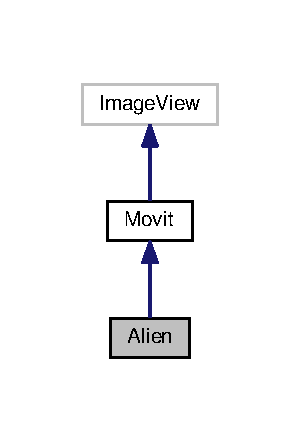
\includegraphics[width=144pt]{class_alien__inherit__graph}
\end{center}
\end{figure}


Graphe de collaboration de Alien\-:
\nopagebreak
\begin{figure}[H]
\begin{center}
\leavevmode
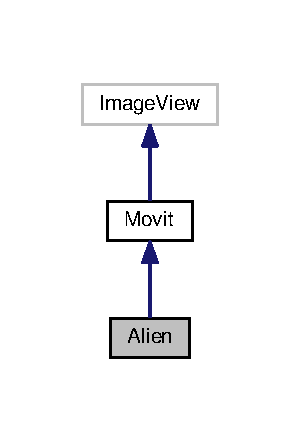
\includegraphics[width=144pt]{class_alien__coll__graph}
\end{center}
\end{figure}
\subsection*{Fonctions membres publiques}
\begin{DoxyCompactItemize}
\item 
\hyperlink{class_alien_a330e393dc37d83b31ff5b0cc7bcd33c8}{Alien} (byte index, double x, double y)
\begin{DoxyCompactList}\small\item\em Constructeur d'un alien. \end{DoxyCompactList}\item 
Boolean \hyperlink{class_alien_ad09b7f992dd6c43fa713e54ce5e00c6a}{collide} (\hyperlink{class_player}{Player} p)
\begin{DoxyCompactList}\small\item\em Méthode détectant la collision avec un alien. \end{DoxyCompactList}\item 
void \hyperlink{class_alien_afd48e2f5c93af1286f24a6caacd84919}{proceed} ()
\begin{DoxyCompactList}\small\item\em Méthode actualisant la position d'un alien. \end{DoxyCompactList}\item 
void \hyperlink{class_alien_a20b62f53c3fb13b489da812ab0bd5941}{shoot} ()
\begin{DoxyCompactList}\small\item\em Méthode créant un tir d'alien avec lancement du son. \end{DoxyCompactList}\item 
void \hyperlink{class_alien_a1d6a17c91905b3e3003edd07fd9210dc}{destruct} ()
\begin{DoxyCompactList}\small\item\em Méthode appelée lors de la destruction d'un alien. \end{DoxyCompactList}\item 
Boolean \hyperlink{class_alien_a7fd4cc9ee380d3bc3a31a9b39600d777}{get\-Destroy} ()
\begin{DoxyCompactList}\small\item\em Méthode renvoyant le drapeau indiquant si l'alien doit être détruit. \end{DoxyCompactList}\item 
double \hyperlink{class_alien_a006b25db50a54b9cbea4d901ffdd8f82}{get\-Vec\-Y} ()
\begin{DoxyCompactList}\small\item\em Méthode renvoyant la position en Y d'un missile. \end{DoxyCompactList}\end{DoxyCompactItemize}
\subsection*{Fonctions membres publiques statiques}
\begin{DoxyCompactItemize}
\item 
static Array\-List$<$ \hyperlink{class_alien}{Alien} $>$ \hyperlink{class_alien_a728d462c9cc08f7ff5f05fb615b73d90}{init} ()
\begin{DoxyCompactList}\small\item\em Liste de tous les aliens. \end{DoxyCompactList}\item 
static void \hyperlink{class_alien_a31f78c3f88539292bd6dc386d573229f}{proceed} (float timestep)
\begin{DoxyCompactList}\small\item\em Méthode actualisant l'état de tous les aliens. \end{DoxyCompactList}\item 
static void \hyperlink{class_alien_a4590038c5fbebdff0478d3436c86fa57}{addnewline} (byte index, double y)
\begin{DoxyCompactList}\small\item\em Méthode rajoutant une ligne d'aliens en haut de l'écran lorsqu'il y a de la place. \end{DoxyCompactList}\item 
static float \hyperlink{class_alien_af08813497b68cf8a37fe1fb102e8ff49}{get\-Delay\-Tir} ()
\begin{DoxyCompactList}\small\item\em Méthode renvoyant le delai entre deux tirs. \end{DoxyCompactList}\item 
static void \hyperlink{class_alien_a3a95e4b5e9e78e0d2355fd344b887569}{set\-Delay\-Tir} (float delay)
\begin{DoxyCompactList}\small\item\em Méthode modifiant le delai entre deux tirs. \end{DoxyCompactList}\item 
static void \hyperlink{class_alien_ae9744d3b25e37ce733608ebd6ef4a789}{reset\-Vitesse} ()
\begin{DoxyCompactList}\small\item\em Méthode réinitialisant la vitesse des aliens. \end{DoxyCompactList}\end{DoxyCompactItemize}
\subsection*{Membres hérités additionnels}


\subsection{Description détaillée}


Définition à la ligne 15 du fichier Alien.\-java.



\subsection{Documentation des constructeurs et destructeur}
\hypertarget{class_alien_a330e393dc37d83b31ff5b0cc7bcd33c8}{\index{Alien@{Alien}!Alien@{Alien}}
\index{Alien@{Alien}!Alien@{Alien}}
\subsubsection[{Alien}]{\setlength{\rightskip}{0pt plus 5cm}Alien.\-Alien (
\begin{DoxyParamCaption}
\item[{byte}]{index, }
\item[{double}]{x, }
\item[{double}]{y}
\end{DoxyParamCaption}
)}}\label{class_alien_a330e393dc37d83b31ff5b0cc7bcd33c8}


Constructeur d'un alien. 

Appelle le constructeur de \hyperlink{class_movit}{Movit}, l'alien aura pour commencer une vitesse vertical nul et une vitesse horizontale positive (il démarre donc en se déplaçant vers la droite). Met destroy à false et donne à l'alien une valeur (score) correspondant à son index dans la liste d'images. 

Définition à la ligne 45 du fichier Alien.\-java.



Voici le graphe des appelants de cette fonction \-:
\nopagebreak
\begin{figure}[H]
\begin{center}
\leavevmode
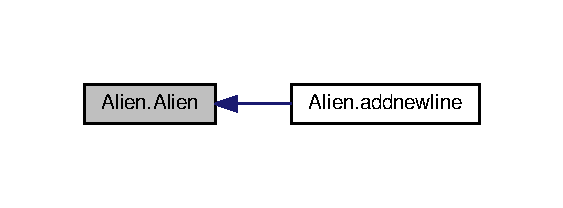
\includegraphics[width=270pt]{class_alien_a330e393dc37d83b31ff5b0cc7bcd33c8_icgraph}
\end{center}
\end{figure}




\subsection{Documentation des fonctions membres}
\hypertarget{class_alien_a4590038c5fbebdff0478d3436c86fa57}{\index{Alien@{Alien}!addnewline@{addnewline}}
\index{addnewline@{addnewline}!Alien@{Alien}}
\subsubsection[{addnewline}]{\setlength{\rightskip}{0pt plus 5cm}static void Alien.\-addnewline (
\begin{DoxyParamCaption}
\item[{byte}]{index, }
\item[{double}]{y}
\end{DoxyParamCaption}
)\hspace{0.3cm}{\ttfamily [static]}}}\label{class_alien_a4590038c5fbebdff0478d3436c86fa57}


Méthode rajoutant une ligne d'aliens en haut de l'écran lorsqu'il y a de la place. 

Cherche l'alien avec l'abcisse la plus petite pour faire démarrer la ligne d'aliens au même x. Puis fait une boucle qui va placer les aliens un à un avec le bon écart et au y précisé en argument. Si la position horizontale s'apprête à dépasser le cadre du jeu, place les aliens qui manquent à gauche du premier qui a été placé. 

Définition à la ligne 154 du fichier Alien.\-java.



Voici le graphe d'appel pour cette fonction \-:
\nopagebreak
\begin{figure}[H]
\begin{center}
\leavevmode
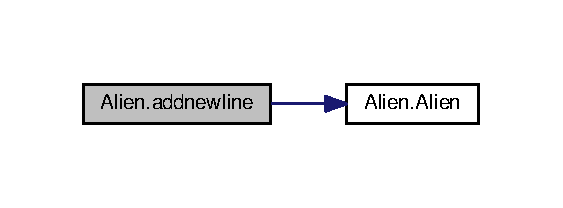
\includegraphics[width=270pt]{class_alien_a4590038c5fbebdff0478d3436c86fa57_cgraph}
\end{center}
\end{figure}


\hypertarget{class_alien_ad09b7f992dd6c43fa713e54ce5e00c6a}{\index{Alien@{Alien}!collide@{collide}}
\index{collide@{collide}!Alien@{Alien}}
\subsubsection[{collide}]{\setlength{\rightskip}{0pt plus 5cm}Boolean Alien.\-collide (
\begin{DoxyParamCaption}
\item[{{\bf Player}}]{p}
\end{DoxyParamCaption}
)}}\label{class_alien_ad09b7f992dd6c43fa713e54ce5e00c6a}


Méthode détectant la collision avec un alien. 

Vérifie d'abord si l'alien n'a pas dépassé le bas de la fenêtre (675px), puis appelle la méthode générale de collision du moteur pour voir si un alien est entré en collision avec le joueur. Renvoi vrai si l'un deux tests est vrai. 

Définition à la ligne 86 du fichier Alien.\-java.



Voici le graphe d'appel pour cette fonction \-:
\nopagebreak
\begin{figure}[H]
\begin{center}
\leavevmode
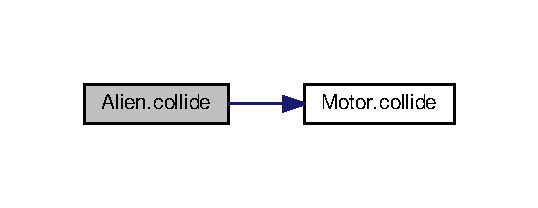
\includegraphics[width=258pt]{class_alien_ad09b7f992dd6c43fa713e54ce5e00c6a_cgraph}
\end{center}
\end{figure}




Voici le graphe des appelants de cette fonction \-:
\nopagebreak
\begin{figure}[H]
\begin{center}
\leavevmode
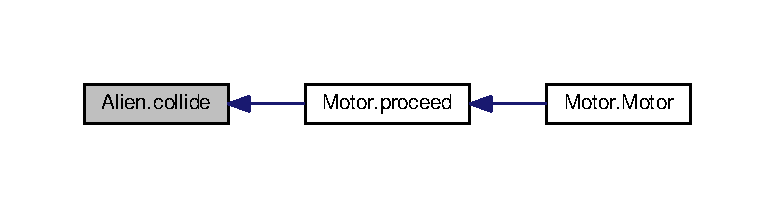
\includegraphics[width=350pt]{class_alien_ad09b7f992dd6c43fa713e54ce5e00c6a_icgraph}
\end{center}
\end{figure}


\hypertarget{class_alien_a1d6a17c91905b3e3003edd07fd9210dc}{\index{Alien@{Alien}!destruct@{destruct}}
\index{destruct@{destruct}!Alien@{Alien}}
\subsubsection[{destruct}]{\setlength{\rightskip}{0pt plus 5cm}void Alien.\-destruct (
\begin{DoxyParamCaption}
{}
\end{DoxyParamCaption}
)}}\label{class_alien_a1d6a17c91905b3e3003edd07fd9210dc}


Méthode appelée lors de la destruction d'un alien. 

Ajoute la valeur de l'alien au score de la partie. Met le témoin de destruction de l'alien à vrai pour que le moteur du jeu sache qu'il faut le détruire. Décrémente le compteur du nombre d'alien. A une probabilité de 1/8 d'ajouter un bonus au jeu en appelant le constructeur de \hyperlink{class_bonus}{Bonus}. 

Définition à la ligne 216 du fichier Alien.\-java.

\hypertarget{class_alien_af08813497b68cf8a37fe1fb102e8ff49}{\index{Alien@{Alien}!get\-Delay\-Tir@{get\-Delay\-Tir}}
\index{get\-Delay\-Tir@{get\-Delay\-Tir}!Alien@{Alien}}
\subsubsection[{get\-Delay\-Tir}]{\setlength{\rightskip}{0pt plus 5cm}static float Alien.\-get\-Delay\-Tir (
\begin{DoxyParamCaption}
{}
\end{DoxyParamCaption}
)\hspace{0.3cm}{\ttfamily [static]}}}\label{class_alien_af08813497b68cf8a37fe1fb102e8ff49}


Méthode renvoyant le delai entre deux tirs. 



Définition à la ligne 248 du fichier Alien.\-java.

\hypertarget{class_alien_a7fd4cc9ee380d3bc3a31a9b39600d777}{\index{Alien@{Alien}!get\-Destroy@{get\-Destroy}}
\index{get\-Destroy@{get\-Destroy}!Alien@{Alien}}
\subsubsection[{get\-Destroy}]{\setlength{\rightskip}{0pt plus 5cm}Boolean Alien.\-get\-Destroy (
\begin{DoxyParamCaption}
{}
\end{DoxyParamCaption}
)}}\label{class_alien_a7fd4cc9ee380d3bc3a31a9b39600d777}


Méthode renvoyant le drapeau indiquant si l'alien doit être détruit. 



Définition à la ligne 236 du fichier Alien.\-java.



Voici le graphe des appelants de cette fonction \-:
\nopagebreak
\begin{figure}[H]
\begin{center}
\leavevmode
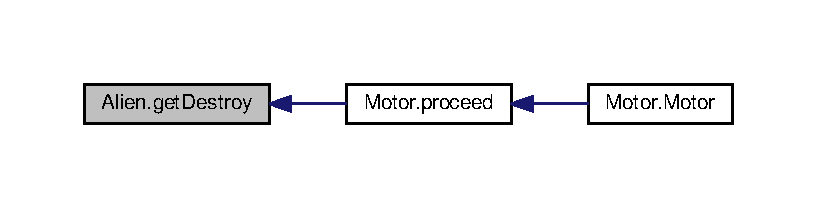
\includegraphics[width=350pt]{class_alien_a7fd4cc9ee380d3bc3a31a9b39600d777_icgraph}
\end{center}
\end{figure}


\hypertarget{class_alien_a006b25db50a54b9cbea4d901ffdd8f82}{\index{Alien@{Alien}!get\-Vec\-Y@{get\-Vec\-Y}}
\index{get\-Vec\-Y@{get\-Vec\-Y}!Alien@{Alien}}
\subsubsection[{get\-Vec\-Y}]{\setlength{\rightskip}{0pt plus 5cm}double Alien.\-get\-Vec\-Y (
\begin{DoxyParamCaption}
{}
\end{DoxyParamCaption}
)}}\label{class_alien_a006b25db50a54b9cbea4d901ffdd8f82}


Méthode renvoyant la position en Y d'un missile. 



Définition à la ligne 242 du fichier Alien.\-java.

\hypertarget{class_alien_a728d462c9cc08f7ff5f05fb615b73d90}{\index{Alien@{Alien}!init@{init}}
\index{init@{init}!Alien@{Alien}}
\subsubsection[{init}]{\setlength{\rightskip}{0pt plus 5cm}static Array\-List$<${\bf Alien}$>$ Alien.\-init (
\begin{DoxyParamCaption}
{}
\end{DoxyParamCaption}
)\hspace{0.3cm}{\ttfamily [static]}}}\label{class_alien_a728d462c9cc08f7ff5f05fb615b73d90}


Liste de tous les aliens. 

Initialise le son joué lors du tir d'une alien et remet les différents délais et vitesses de la classe à leur valeurs initiales. Initialise la liste d'aliens du jeu et appelle le constructeur 5$\ast$11 fois en plaçant chaque alien à sa position (55 pixels entre chaque aliens côte à côte, 50 pixels entre chaque lignes d'aliens). Les aliens sont ajoutés de bas en haut pour que le dernier alien de la liste soit toujours dans la ligne la plus haute (sert pour l'ajout de nouvelles lignes). Initialise le compteur du nombre d'aliens et ajoute une méthode dynamique qui augmente la vitesse des ennemis (et donc la difficulté du jeu) à chaque fois que ce compteur change de valeur. Renvoie la liste ainsi crée. 

Définition à la ligne 60 du fichier Alien.\-java.



Voici le graphe d'appel pour cette fonction \-:
\nopagebreak
\begin{figure}[H]
\begin{center}
\leavevmode
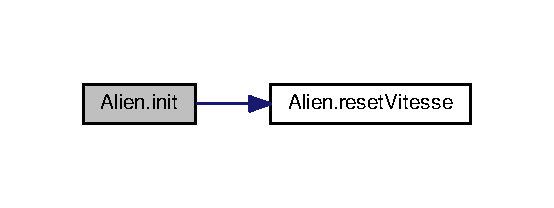
\includegraphics[width=266pt]{class_alien_a728d462c9cc08f7ff5f05fb615b73d90_cgraph}
\end{center}
\end{figure}


\hypertarget{class_alien_afd48e2f5c93af1286f24a6caacd84919}{\index{Alien@{Alien}!proceed@{proceed}}
\index{proceed@{proceed}!Alien@{Alien}}
\subsubsection[{proceed}]{\setlength{\rightskip}{0pt plus 5cm}void Alien.\-proceed (
\begin{DoxyParamCaption}
{}
\end{DoxyParamCaption}
)}}\label{class_alien_afd48e2f5c93af1286f24a6caacd84919}


Méthode actualisant la position d'un alien. 

Ajoute à la position de l'alien ses vitesses horizontale et verticale. 

Définition à la ligne 104 du fichier Alien.\-java.

\hypertarget{class_alien_a31f78c3f88539292bd6dc386d573229f}{\index{Alien@{Alien}!proceed@{proceed}}
\index{proceed@{proceed}!Alien@{Alien}}
\subsubsection[{proceed}]{\setlength{\rightskip}{0pt plus 5cm}static void Alien.\-proceed (
\begin{DoxyParamCaption}
\item[{float}]{timestep}
\end{DoxyParamCaption}
)\hspace{0.3cm}{\ttfamily [static]}}}\label{class_alien_a31f78c3f88539292bd6dc386d573229f}


Méthode actualisant l'état de tous les aliens. 

Pour chaque alien, met à jour ses vitesses horizontale et verticale \-: Si la vitesse horizontale est à 0.\-0, alors les aliens viennent de descendre d'une ligne, cette fonction remet donc la vitesse verticale à 0.\-0 et remet la vitesse horizontale à sa valeur générale vitesse\-X. Sinon vérifie si au prochain déplacement, un alien va dépasser le cadre du jeu, si c'est le cas, met la vitesse horizontale à 0.\-0, la vitesse verticale à vitesse\-Y (pour que le prochain déplacement des aliens soit de les faire descendre), et inverse vitesse\-X pour qu'au tour de boucle suivant, les aliens se déplacent dans l'autre direction. Enfin, met à jour le delai général en fonction du temps qui s'est écoulé depuis le dernier \hyperlink{class_alien_afd48e2f5c93af1286f24a6caacd84919}{proceed()}, et si le délai est suffisant, fait tirer un alien. 

Définition à la ligne 117 du fichier Alien.\-java.



Voici le graphe d'appel pour cette fonction \-:
\nopagebreak
\begin{figure}[H]
\begin{center}
\leavevmode
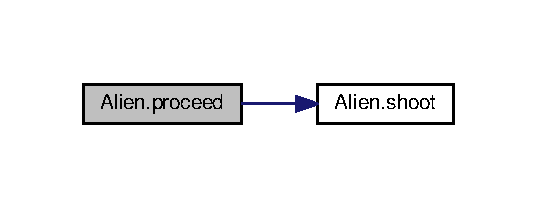
\includegraphics[width=258pt]{class_alien_a31f78c3f88539292bd6dc386d573229f_cgraph}
\end{center}
\end{figure}


\hypertarget{class_alien_ae9744d3b25e37ce733608ebd6ef4a789}{\index{Alien@{Alien}!reset\-Vitesse@{reset\-Vitesse}}
\index{reset\-Vitesse@{reset\-Vitesse}!Alien@{Alien}}
\subsubsection[{reset\-Vitesse}]{\setlength{\rightskip}{0pt plus 5cm}static void Alien.\-reset\-Vitesse (
\begin{DoxyParamCaption}
{}
\end{DoxyParamCaption}
)\hspace{0.3cm}{\ttfamily [static]}}}\label{class_alien_ae9744d3b25e37ce733608ebd6ef4a789}


Méthode réinitialisant la vitesse des aliens. 

Remet la vitesse des aliens à leur valeurs initiales, utilisée en cas de nouvelle partie. 

Définition à la ligne 262 du fichier Alien.\-java.



Voici le graphe des appelants de cette fonction \-:
\nopagebreak
\begin{figure}[H]
\begin{center}
\leavevmode
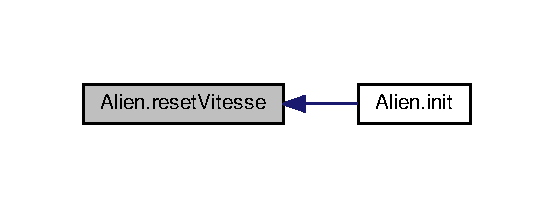
\includegraphics[width=266pt]{class_alien_ae9744d3b25e37ce733608ebd6ef4a789_icgraph}
\end{center}
\end{figure}


\hypertarget{class_alien_a3a95e4b5e9e78e0d2355fd344b887569}{\index{Alien@{Alien}!set\-Delay\-Tir@{set\-Delay\-Tir}}
\index{set\-Delay\-Tir@{set\-Delay\-Tir}!Alien@{Alien}}
\subsubsection[{set\-Delay\-Tir}]{\setlength{\rightskip}{0pt plus 5cm}static void Alien.\-set\-Delay\-Tir (
\begin{DoxyParamCaption}
\item[{float}]{delay}
\end{DoxyParamCaption}
)\hspace{0.3cm}{\ttfamily [static]}}}\label{class_alien_a3a95e4b5e9e78e0d2355fd344b887569}


Méthode modifiant le delai entre deux tirs. 



Définition à la ligne 254 du fichier Alien.\-java.

\hypertarget{class_alien_a20b62f53c3fb13b489da812ab0bd5941}{\index{Alien@{Alien}!shoot@{shoot}}
\index{shoot@{shoot}!Alien@{Alien}}
\subsubsection[{shoot}]{\setlength{\rightskip}{0pt plus 5cm}void Alien.\-shoot (
\begin{DoxyParamCaption}
{}
\end{DoxyParamCaption}
)}}\label{class_alien_a20b62f53c3fb13b489da812ab0bd5941}


Méthode créant un tir d'alien avec lancement du son. 

Ajoute un tir à liste des tirs en appelant le constructeur de \hyperlink{class_tir}{Tir} en fonction de la position de l'alien qui tire (le tire sera positionné juste en dessous et au centre de l'alien) et de la vitesse de tir de cette classe. 

Définition à la ligne 180 du fichier Alien.\-java.



Voici le graphe des appelants de cette fonction \-:
\nopagebreak
\begin{figure}[H]
\begin{center}
\leavevmode
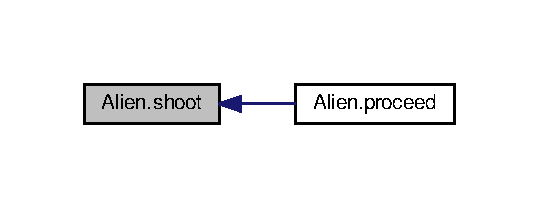
\includegraphics[width=258pt]{class_alien_a20b62f53c3fb13b489da812ab0bd5941_icgraph}
\end{center}
\end{figure}




La documentation de cette classe a été générée à partir du fichier suivant \-:\begin{DoxyCompactItemize}
\item 
\hyperlink{_alien_8java}{Alien.\-java}\end{DoxyCompactItemize}

\hypertarget{class_bonus}{\section{Référence de la classe Bonus}
\label{class_bonus}\index{Bonus@{Bonus}}
}


Graphe d'héritage de Bonus\-:
\nopagebreak
\begin{figure}[H]
\begin{center}
\leavevmode
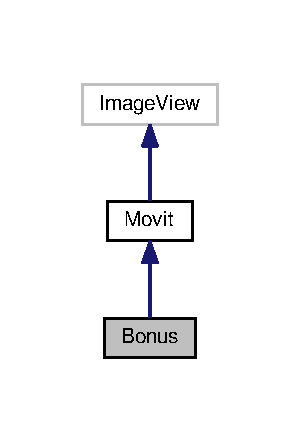
\includegraphics[width=144pt]{class_bonus__inherit__graph}
\end{center}
\end{figure}


Graphe de collaboration de Bonus\-:
\nopagebreak
\begin{figure}[H]
\begin{center}
\leavevmode
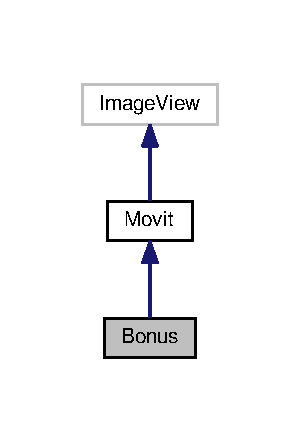
\includegraphics[width=144pt]{class_bonus__coll__graph}
\end{center}
\end{figure}
\subsection*{Fonctions membres publiques}
\begin{DoxyCompactItemize}
\item 
\hyperlink{class_bonus_a1d1e2ebe69d7e1ac68e2550f80d2e632}{Bonus} (double x, double y)
\begin{DoxyCompactList}\small\item\em Constructeur d'un bonus. \end{DoxyCompactList}\item 
Boolean \hyperlink{class_bonus_a09f19db4fdca514ddb4b526c4ed4cc4f}{collide} (\hyperlink{class_player}{Player} p)
\begin{DoxyCompactList}\small\item\em Méthode détectant la collision entre bonus et joueur. \end{DoxyCompactList}\item 
void \hyperlink{class_bonus_a42e90885234abf53398e0c5d0b47cf0d}{proceed} ()
\begin{DoxyCompactList}\small\item\em Méthode actualisant la position d'un bonus. \end{DoxyCompactList}\item 
void \hyperlink{class_bonus_a3082cd3a33dee61d0d3d28727508f834}{add\-Time\-Step} (float timestep)
\begin{DoxyCompactList}\small\item\em Méthode ajoutant le temps écoulé (timestep) au chronomètre d'activation du bonus. \end{DoxyCompactList}\item 
void \hyperlink{class_bonus_ae3818b4a920609eecb9e0be60cd7afc9}{active} ()
\begin{DoxyCompactList}\small\item\em Méthode appelée à l'activation du bonus. \end{DoxyCompactList}\item 
void \hyperlink{class_bonus_a43bd71425625417a8c37e919510f90c3}{inactive} ()
\begin{DoxyCompactList}\small\item\em Méthode appelée à la désactivation du bonus. \end{DoxyCompactList}\item 
float \hyperlink{class_bonus_a2912fd692ce4fe1a7b34c4fa14c8fe9f}{get\-Time} ()
\begin{DoxyCompactList}\small\item\em Méthode retournant le temps écoulé depuis que le bonus s'est activé \end{DoxyCompactList}\end{DoxyCompactItemize}
\subsection*{Attributs publics statiques}
\begin{DoxyCompactItemize}
\item 
static double \hyperlink{class_bonus_a7ae08569114898b429584cbcec091c4d}{M\-A\-X\-T\-I\-M\-E} =10.\-0
\begin{DoxyCompactList}\small\item\em Temps maximum durant lequel un bonus est actif. \end{DoxyCompactList}\item 
static int \hyperlink{class_bonus_a62d1d7bef5df2d449bc67e1fb1985b5f}{S\-C\-O\-R\-E\-U\-P} =200
\begin{DoxyCompactList}\small\item\em Score apporté par le bonus \char`\"{}score\char`\"{}. \end{DoxyCompactList}\item 
static int \hyperlink{class_bonus_ab84109f50f0520fbfb36973c7e937528}{D\-I\-S\-T\-R\-E\-C\-U\-L\-E} =200
\begin{DoxyCompactList}\small\item\em Distance de recul des ennemis causée par le bonus \char`\"{}recul\char`\"{}. \end{DoxyCompactList}\end{DoxyCompactItemize}
\subsection*{Membres hérités additionnels}


\subsection{Description détaillée}


Définition à la ligne 17 du fichier Bonus.\-java.



\subsection{Documentation des constructeurs et destructeur}
\hypertarget{class_bonus_a1d1e2ebe69d7e1ac68e2550f80d2e632}{\index{Bonus@{Bonus}!Bonus@{Bonus}}
\index{Bonus@{Bonus}!Bonus@{Bonus}}
\subsubsection[{Bonus}]{\setlength{\rightskip}{0pt plus 5cm}Bonus.\-Bonus (
\begin{DoxyParamCaption}
\item[{double}]{x, }
\item[{double}]{y}
\end{DoxyParamCaption}
)}}\label{class_bonus_a1d1e2ebe69d7e1ac68e2550f80d2e632}


Constructeur d'un bonus. 

Appelle le constructeur de \hyperlink{class_movit}{Movit} en utilisant une image de bonus choisie au hasard. Diminue la position en X de la moitié de la largeur de l'image du bonus (pour que le bonus apparaisse au milieu de l'alien qui l'a lâché). Récupère l'index de l'image du bonus qui a été choisie au hasard pour pouvoir l'identifier. Récupère la paire d'effet in/actif de l'effet correspondant à l'index et les attribue respectivement à leur variable. Initialise le chronomètre à 0.\-0 . 

Définition à la ligne 48 du fichier Bonus.\-java.



\subsection{Documentation des fonctions membres}
\hypertarget{class_bonus_ae3818b4a920609eecb9e0be60cd7afc9}{\index{Bonus@{Bonus}!active@{active}}
\index{active@{active}!Bonus@{Bonus}}
\subsubsection[{active}]{\setlength{\rightskip}{0pt plus 5cm}void Bonus.\-active (
\begin{DoxyParamCaption}
{}
\end{DoxyParamCaption}
)}}\label{class_bonus_ae3818b4a920609eecb9e0be60cd7afc9}


Méthode appelée à l'activation du bonus. 

Lance l'Effet \char`\"{}actif\char`\"{} du bonus puis rajoute ce bonus à la liste d'effets en cours d'activation. 

Définition à la ligne 166 du fichier Bonus.\-java.

\hypertarget{class_bonus_a3082cd3a33dee61d0d3d28727508f834}{\index{Bonus@{Bonus}!add\-Time\-Step@{add\-Time\-Step}}
\index{add\-Time\-Step@{add\-Time\-Step}!Bonus@{Bonus}}
\subsubsection[{add\-Time\-Step}]{\setlength{\rightskip}{0pt plus 5cm}void Bonus.\-add\-Time\-Step (
\begin{DoxyParamCaption}
\item[{float}]{timestep}
\end{DoxyParamCaption}
)}}\label{class_bonus_a3082cd3a33dee61d0d3d28727508f834}


Méthode ajoutant le temps écoulé (timestep) au chronomètre d'activation du bonus. 



Définition à la ligne 89 du fichier Bonus.\-java.

\hypertarget{class_bonus_a09f19db4fdca514ddb4b526c4ed4cc4f}{\index{Bonus@{Bonus}!collide@{collide}}
\index{collide@{collide}!Bonus@{Bonus}}
\subsubsection[{collide}]{\setlength{\rightskip}{0pt plus 5cm}Boolean Bonus.\-collide (
\begin{DoxyParamCaption}
\item[{{\bf Player}}]{p}
\end{DoxyParamCaption}
)}}\label{class_bonus_a09f19db4fdca514ddb4b526c4ed4cc4f}


Méthode détectant la collision entre bonus et joueur. 

Appelle la fonction \hyperlink{class_bonus_a09f19db4fdca514ddb4b526c4ed4cc4f}{collide()} du moteur pour voir si une collision s'est produite entre l'image du bonus et du joueur. Joue un son si le joueur a attrapé le bonus. Renvoie vrai ou faux en fonction. 

Définition à la ligne 64 du fichier Bonus.\-java.



Voici le graphe d'appel pour cette fonction \-:
\nopagebreak
\begin{figure}[H]
\begin{center}
\leavevmode
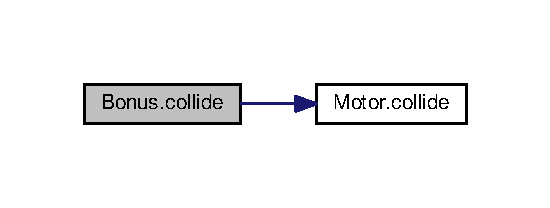
\includegraphics[width=264pt]{class_bonus_a09f19db4fdca514ddb4b526c4ed4cc4f_cgraph}
\end{center}
\end{figure}




Voici le graphe des appelants de cette fonction \-:
\nopagebreak
\begin{figure}[H]
\begin{center}
\leavevmode
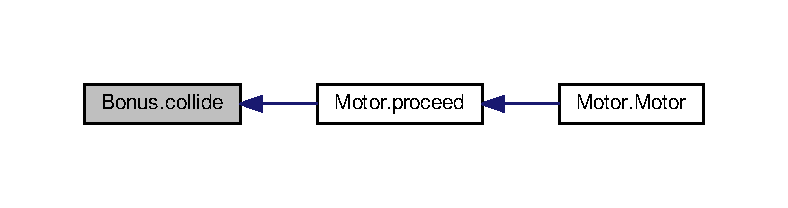
\includegraphics[width=350pt]{class_bonus_a09f19db4fdca514ddb4b526c4ed4cc4f_icgraph}
\end{center}
\end{figure}


\hypertarget{class_bonus_a2912fd692ce4fe1a7b34c4fa14c8fe9f}{\index{Bonus@{Bonus}!get\-Time@{get\-Time}}
\index{get\-Time@{get\-Time}!Bonus@{Bonus}}
\subsubsection[{get\-Time}]{\setlength{\rightskip}{0pt plus 5cm}float Bonus.\-get\-Time (
\begin{DoxyParamCaption}
{}
\end{DoxyParamCaption}
)}}\label{class_bonus_a2912fd692ce4fe1a7b34c4fa14c8fe9f}


Méthode retournant le temps écoulé depuis que le bonus s'est activé 



Définition à la ligne 190 du fichier Bonus.\-java.



Voici le graphe des appelants de cette fonction \-:
\nopagebreak
\begin{figure}[H]
\begin{center}
\leavevmode
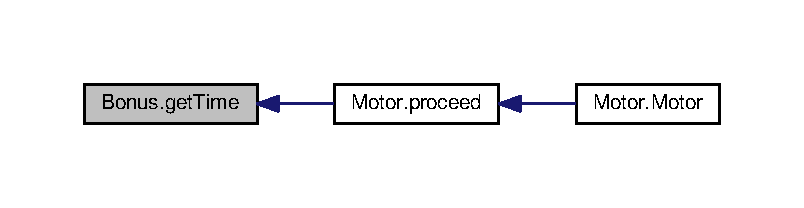
\includegraphics[width=350pt]{class_bonus_a2912fd692ce4fe1a7b34c4fa14c8fe9f_icgraph}
\end{center}
\end{figure}


\hypertarget{class_bonus_a43bd71425625417a8c37e919510f90c3}{\index{Bonus@{Bonus}!inactive@{inactive}}
\index{inactive@{inactive}!Bonus@{Bonus}}
\subsubsection[{inactive}]{\setlength{\rightskip}{0pt plus 5cm}void Bonus.\-inactive (
\begin{DoxyParamCaption}
{}
\end{DoxyParamCaption}
)}}\label{class_bonus_a43bd71425625417a8c37e919510f90c3}


Méthode appelée à la désactivation du bonus. 

Lance l'Effet \char`\"{}inactif\char`\"{} du bonus. 

Définition à la ligne 175 du fichier Bonus.\-java.

\hypertarget{class_bonus_a42e90885234abf53398e0c5d0b47cf0d}{\index{Bonus@{Bonus}!proceed@{proceed}}
\index{proceed@{proceed}!Bonus@{Bonus}}
\subsubsection[{proceed}]{\setlength{\rightskip}{0pt plus 5cm}void Bonus.\-proceed (
\begin{DoxyParamCaption}
{}
\end{DoxyParamCaption}
)}}\label{class_bonus_a42e90885234abf53398e0c5d0b47cf0d}


Méthode actualisant la position d'un bonus. 

Ajoute à l'ordonné du bonus sa vitesse verticale. Le bonus ne chutant que vers le bas, il n'a pas de déplacement horizontal. 

Définition à la ligne 83 du fichier Bonus.\-java.



\subsection{Documentation des données membres}
\hypertarget{class_bonus_ab84109f50f0520fbfb36973c7e937528}{\index{Bonus@{Bonus}!D\-I\-S\-T\-R\-E\-C\-U\-L\-E@{D\-I\-S\-T\-R\-E\-C\-U\-L\-E}}
\index{D\-I\-S\-T\-R\-E\-C\-U\-L\-E@{D\-I\-S\-T\-R\-E\-C\-U\-L\-E}!Bonus@{Bonus}}
\subsubsection[{D\-I\-S\-T\-R\-E\-C\-U\-L\-E}]{\setlength{\rightskip}{0pt plus 5cm}int Bonus.\-D\-I\-S\-T\-R\-E\-C\-U\-L\-E =200\hspace{0.3cm}{\ttfamily [static]}}}\label{class_bonus_ab84109f50f0520fbfb36973c7e937528}


Distance de recul des ennemis causée par le bonus \char`\"{}recul\char`\"{}. 


\begin{DoxyItemize}
\item 
\end{DoxyItemize}

Définition à la ligne 29 du fichier Bonus.\-java.

\hypertarget{class_bonus_a7ae08569114898b429584cbcec091c4d}{\index{Bonus@{Bonus}!M\-A\-X\-T\-I\-M\-E@{M\-A\-X\-T\-I\-M\-E}}
\index{M\-A\-X\-T\-I\-M\-E@{M\-A\-X\-T\-I\-M\-E}!Bonus@{Bonus}}
\subsubsection[{M\-A\-X\-T\-I\-M\-E}]{\setlength{\rightskip}{0pt plus 5cm}double Bonus.\-M\-A\-X\-T\-I\-M\-E =10.\-0\hspace{0.3cm}{\ttfamily [static]}}}\label{class_bonus_a7ae08569114898b429584cbcec091c4d}


Temps maximum durant lequel un bonus est actif. 


\begin{DoxyItemize}
\item 
\end{DoxyItemize}

Définition à la ligne 25 du fichier Bonus.\-java.

\hypertarget{class_bonus_a62d1d7bef5df2d449bc67e1fb1985b5f}{\index{Bonus@{Bonus}!S\-C\-O\-R\-E\-U\-P@{S\-C\-O\-R\-E\-U\-P}}
\index{S\-C\-O\-R\-E\-U\-P@{S\-C\-O\-R\-E\-U\-P}!Bonus@{Bonus}}
\subsubsection[{S\-C\-O\-R\-E\-U\-P}]{\setlength{\rightskip}{0pt plus 5cm}int Bonus.\-S\-C\-O\-R\-E\-U\-P =200\hspace{0.3cm}{\ttfamily [static]}}}\label{class_bonus_a62d1d7bef5df2d449bc67e1fb1985b5f}


Score apporté par le bonus \char`\"{}score\char`\"{}. 


\begin{DoxyItemize}
\item 
\end{DoxyItemize}

Définition à la ligne 27 du fichier Bonus.\-java.



La documentation de cette classe a été générée à partir du fichier suivant \-:\begin{DoxyCompactItemize}
\item 
\hyperlink{_bonus_8java}{Bonus.\-java}\end{DoxyCompactItemize}

\hypertarget{class_game}{\section{Référence de la classe Game}
\label{class_game}\index{Game@{Game}}
}


Graphe d'héritage de Game\-:
\nopagebreak
\begin{figure}[H]
\begin{center}
\leavevmode
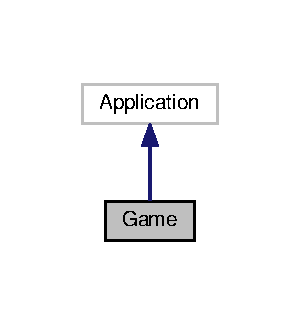
\includegraphics[width=144pt]{class_game__inherit__graph}
\end{center}
\end{figure}


Graphe de collaboration de Game\-:
\nopagebreak
\begin{figure}[H]
\begin{center}
\leavevmode
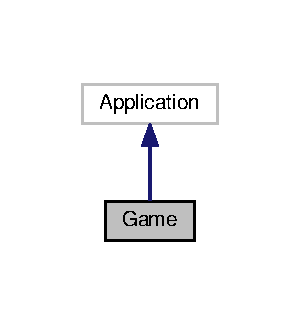
\includegraphics[width=144pt]{class_game__coll__graph}
\end{center}
\end{figure}
\subsection*{Fonctions membres publiques}
\begin{DoxyCompactItemize}
\item 
void \hyperlink{class_game_af537a745b82fdda8087d19cb61abb043}{start} (Stage jeu)
\begin{DoxyCompactList}\small\item\em Méthode principale d'initialisation du jeu. \end{DoxyCompactList}\end{DoxyCompactItemize}
\subsection*{Fonctions membres publiques statiques}
\begin{DoxyCompactItemize}
\item 
static void \hyperlink{class_game_a6820c58e98b057326b794a928352ff8a}{set\-Current\-Level} (int n)
\begin{DoxyCompactList}\small\item\em Methode changeant la valeur de l'écran sur lequel on se trouve. \end{DoxyCompactList}\item 
static \hyperlink{class_motor}{Motor} \hyperlink{class_game_ad2ca85b9da3d4f432e80c4c30d27a04a}{get\-Motor} ()
\begin{DoxyCompactList}\small\item\em Methode renvoyant l'objet \char`\"{}motor\char`\"{} qui représente le moteur du jeu. \end{DoxyCompactList}\item 
static Flow\-Pane \hyperlink{class_game_aa1efcee841a5a0f096b824b1aca2bfb5}{get\-Vie} ()
\begin{DoxyCompactList}\small\item\em Methode renvoyant le conteneur des vies du joueur. \end{DoxyCompactList}\item 
static Text \hyperlink{class_game_a88c9ee21de18322252a578965d6d95d5}{get\-Score} ()
\begin{DoxyCompactList}\small\item\em Methode retournant l'objet Text qui contient le score du joueur. \end{DoxyCompactList}\item 
static Text \hyperlink{class_game_a45ca829175e700eee22814f7692e9224}{get\-Level} ()
\begin{DoxyCompactList}\small\item\em Methode retournant l'objet Text qui contient le niveau auquel est arrivé le joueur. \end{DoxyCompactList}\item 
static void \hyperlink{class_game_ae52595a27ac1b327b05db2129ad81fca}{main} (String\mbox{[}$\,$\mbox{]} args)
\begin{DoxyCompactList}\small\item\em Methode de lancement general du jeu. \end{DoxyCompactList}\end{DoxyCompactItemize}
\subsection*{Attributs publics statiques}
\begin{DoxyCompactItemize}
\item 
static final double \hyperlink{class_game_a717d94203369772a9d40c0efc20eb779}{W\-I\-D\-T\-H} =800
\begin{DoxyCompactList}\small\item\em Largeur de la fenêtre. \end{DoxyCompactList}\item 
static final double \hyperlink{class_game_a11eafdb6df55b7fc6ee0e9d3573052d0}{H\-E\-I\-G\-H\-T} =800
\begin{DoxyCompactList}\small\item\em Hauteur de la fenêtre. \end{DoxyCompactList}\end{DoxyCompactItemize}


\subsection{Description détaillée}


Définition à la ligne 36 du fichier Game.\-java.



\subsection{Documentation des fonctions membres}
\hypertarget{class_game_a45ca829175e700eee22814f7692e9224}{\index{Game@{Game}!get\-Level@{get\-Level}}
\index{get\-Level@{get\-Level}!Game@{Game}}
\subsubsection[{get\-Level}]{\setlength{\rightskip}{0pt plus 5cm}static Text Game.\-get\-Level (
\begin{DoxyParamCaption}
{}
\end{DoxyParamCaption}
)\hspace{0.3cm}{\ttfamily [static]}}}\label{class_game_a45ca829175e700eee22814f7692e9224}


Methode retournant l'objet Text qui contient le niveau auquel est arrivé le joueur. 



Définition à la ligne 426 du fichier Game.\-java.

\hypertarget{class_game_ad2ca85b9da3d4f432e80c4c30d27a04a}{\index{Game@{Game}!get\-Motor@{get\-Motor}}
\index{get\-Motor@{get\-Motor}!Game@{Game}}
\subsubsection[{get\-Motor}]{\setlength{\rightskip}{0pt plus 5cm}static {\bf Motor} Game.\-get\-Motor (
\begin{DoxyParamCaption}
{}
\end{DoxyParamCaption}
)\hspace{0.3cm}{\ttfamily [static]}}}\label{class_game_ad2ca85b9da3d4f432e80c4c30d27a04a}


Methode renvoyant l'objet \char`\"{}motor\char`\"{} qui représente le moteur du jeu. 



Définition à la ligne 408 du fichier Game.\-java.



Voici le graphe des appelants de cette fonction \-:
\nopagebreak
\begin{figure}[H]
\begin{center}
\leavevmode
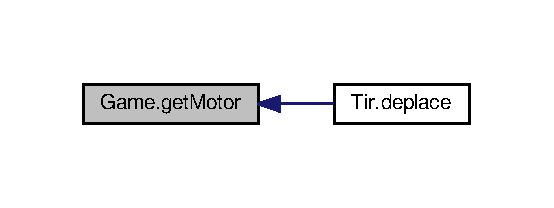
\includegraphics[width=266pt]{class_game_ad2ca85b9da3d4f432e80c4c30d27a04a_icgraph}
\end{center}
\end{figure}


\hypertarget{class_game_a88c9ee21de18322252a578965d6d95d5}{\index{Game@{Game}!get\-Score@{get\-Score}}
\index{get\-Score@{get\-Score}!Game@{Game}}
\subsubsection[{get\-Score}]{\setlength{\rightskip}{0pt plus 5cm}static Text Game.\-get\-Score (
\begin{DoxyParamCaption}
{}
\end{DoxyParamCaption}
)\hspace{0.3cm}{\ttfamily [static]}}}\label{class_game_a88c9ee21de18322252a578965d6d95d5}


Methode retournant l'objet Text qui contient le score du joueur. 



Définition à la ligne 420 du fichier Game.\-java.

\hypertarget{class_game_aa1efcee841a5a0f096b824b1aca2bfb5}{\index{Game@{Game}!get\-Vie@{get\-Vie}}
\index{get\-Vie@{get\-Vie}!Game@{Game}}
\subsubsection[{get\-Vie}]{\setlength{\rightskip}{0pt plus 5cm}static Flow\-Pane Game.\-get\-Vie (
\begin{DoxyParamCaption}
{}
\end{DoxyParamCaption}
)\hspace{0.3cm}{\ttfamily [static]}}}\label{class_game_aa1efcee841a5a0f096b824b1aca2bfb5}


Methode renvoyant le conteneur des vies du joueur. 



Définition à la ligne 414 du fichier Game.\-java.

\hypertarget{class_game_ae52595a27ac1b327b05db2129ad81fca}{\index{Game@{Game}!main@{main}}
\index{main@{main}!Game@{Game}}
\subsubsection[{main}]{\setlength{\rightskip}{0pt plus 5cm}static void Game.\-main (
\begin{DoxyParamCaption}
\item[{String\mbox{[}$\,$\mbox{]}}]{args}
\end{DoxyParamCaption}
)\hspace{0.3cm}{\ttfamily [static]}}}\label{class_game_ae52595a27ac1b327b05db2129ad81fca}


Methode de lancement general du jeu. 



Définition à la ligne 480 du fichier Game.\-java.

\hypertarget{class_game_a6820c58e98b057326b794a928352ff8a}{\index{Game@{Game}!set\-Current\-Level@{set\-Current\-Level}}
\index{set\-Current\-Level@{set\-Current\-Level}!Game@{Game}}
\subsubsection[{set\-Current\-Level}]{\setlength{\rightskip}{0pt plus 5cm}static void Game.\-set\-Current\-Level (
\begin{DoxyParamCaption}
\item[{int}]{n}
\end{DoxyParamCaption}
)\hspace{0.3cm}{\ttfamily [static]}}}\label{class_game_a6820c58e98b057326b794a928352ff8a}


Methode changeant la valeur de l'écran sur lequel on se trouve. 



Définition à la ligne 401 du fichier Game.\-java.



Voici le graphe des appelants de cette fonction \-:
\nopagebreak
\begin{figure}[H]
\begin{center}
\leavevmode
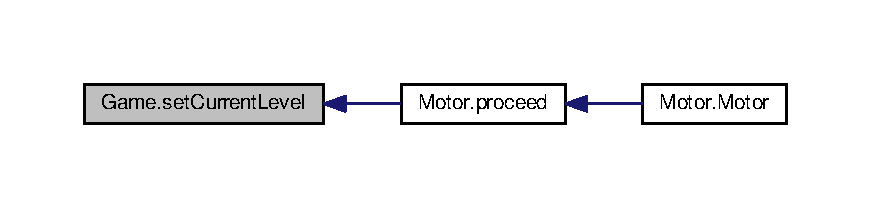
\includegraphics[width=350pt]{class_game_a6820c58e98b057326b794a928352ff8a_icgraph}
\end{center}
\end{figure}


\hypertarget{class_game_af537a745b82fdda8087d19cb61abb043}{\index{Game@{Game}!start@{start}}
\index{start@{start}!Game@{Game}}
\subsubsection[{start}]{\setlength{\rightskip}{0pt plus 5cm}void Game.\-start (
\begin{DoxyParamCaption}
\item[{Stage}]{jeu}
\end{DoxyParamCaption}
)}}\label{class_game_af537a745b82fdda8087d19cb61abb043}


Méthode principale d'initialisation du jeu. 


\begin{DoxyItemize}
\item Empêche le redimensionnement de la fenêtre
\item Fait en sorte que la musique du menu se joue en boucle
\item Ajoute le menu principal à la liste des écrans du jeu
\item Y ajoute la page de règle
\item Y ajoute l'écran de jeu
\item Y ajoute l'écran de pause
\item Y ajoute l'écran de game over
\item Construit la fenêtre de W\-I\-D\-T\-H$\ast$\-H\-E\-I\-G\-H\-T contenant le menu
\item Charge la feuille de style qui sera utilisé pour l'apparence des boutons
\end{DoxyItemize}

Ajoute à l'objet \char`\"{}currentlevel\char`\"{} des événements dynamiques qui se produisent lorsque la valeur de \char`\"{}currentlevel\char`\"{} change. Ainsi les réglages nécessaires en fonction de l'écran qu'on veut afficher se feront automatiquement. Si on vient de quitter l'écran de pause ou de gameover, il faut retirer du conteneur de celui-\/ci de l'écran du jeu pour que ce dernier puisse à nouveau être affiché directement par la fenêtre (seul un conteneur qui n'est contenu par aucun autre peut être utilisé comme conteneur \char`\"{}racine\char`\"{}). Change le conteneur \char`\"{}racine\char`\"{} pour lui donner l'écran correspondant à la nouvelle valeur. Si le nouvel écran est celui du menu ou des règles, lance la musique d'ambiance du menu si ce n'est pas déjà fait, sinon arrête la musique. Si le nouvel écran est celui du jeu, lance le moteur du jeu. Si le nouvel écran est celui de pause ou de gameover, arrête le moteur du jeu puis ajoute l'écran de jeu au conteneur de cet écran (pour que la pause ou le gameover viennent s'afficher par-\/dessus le jeu). Enfin, si le nouvel écran est celui du game over, lance le son du gameover et lance la fonction newgame().

Fait en sorte que lorsqu'une touche du clavier est appuyée, celle-\/ci soit ajoutée dans la liste des touches qui sont passées au moteur. Si une touche du clavier est relâchée, elle est au contraire enlevée de cette même liste. Une exception est faite pour que la touche \char`\"{}Échap\char`\"{}, lorsqu'elle est pressée, fasse revenir au menu principal en jouant le son qui correspond à l'appuie d'un bouton, sauf si le jeu affiche actuellement l'écran de jeu (dans ce cas il faudra passer par la touche \char`\"{}\-P\char`\"{} qui met en pause).

Définition à la ligne 66 du fichier Game.\-java.



\subsection{Documentation des données membres}
\hypertarget{class_game_a11eafdb6df55b7fc6ee0e9d3573052d0}{\index{Game@{Game}!H\-E\-I\-G\-H\-T@{H\-E\-I\-G\-H\-T}}
\index{H\-E\-I\-G\-H\-T@{H\-E\-I\-G\-H\-T}!Game@{Game}}
\subsubsection[{H\-E\-I\-G\-H\-T}]{\setlength{\rightskip}{0pt plus 5cm}final double Game.\-H\-E\-I\-G\-H\-T =800\hspace{0.3cm}{\ttfamily [static]}}}\label{class_game_a11eafdb6df55b7fc6ee0e9d3573052d0}


Hauteur de la fenêtre. 


\begin{DoxyItemize}
\item 
\end{DoxyItemize}

Définition à la ligne 61 du fichier Game.\-java.

\hypertarget{class_game_a717d94203369772a9d40c0efc20eb779}{\index{Game@{Game}!W\-I\-D\-T\-H@{W\-I\-D\-T\-H}}
\index{W\-I\-D\-T\-H@{W\-I\-D\-T\-H}!Game@{Game}}
\subsubsection[{W\-I\-D\-T\-H}]{\setlength{\rightskip}{0pt plus 5cm}final double Game.\-W\-I\-D\-T\-H =800\hspace{0.3cm}{\ttfamily [static]}}}\label{class_game_a717d94203369772a9d40c0efc20eb779}


Largeur de la fenêtre. 


\begin{DoxyItemize}
\item 
\end{DoxyItemize}

Définition à la ligne 59 du fichier Game.\-java.



La documentation de cette classe a été générée à partir du fichier suivant \-:\begin{DoxyCompactItemize}
\item 
\hyperlink{_game_8java}{Game.\-java}\end{DoxyCompactItemize}

\hypertarget{class_house}{\section{Référence de la classe House}
\label{class_house}\index{House@{House}}
}


Graphe d'héritage de House\-:
\nopagebreak
\begin{figure}[H]
\begin{center}
\leavevmode
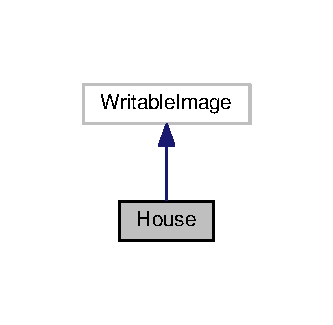
\includegraphics[width=160pt]{class_house__inherit__graph}
\end{center}
\end{figure}


Graphe de collaboration de House\-:
\nopagebreak
\begin{figure}[H]
\begin{center}
\leavevmode
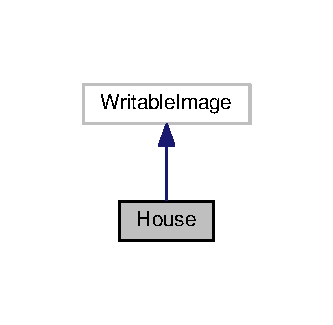
\includegraphics[width=160pt]{class_house__coll__graph}
\end{center}
\end{figure}
\subsection*{Fonctions membres publiques}
\begin{DoxyCompactItemize}
\item 
\hyperlink{class_house_aec83bd8191e1fa3ea56f7428445cc78a}{House} (int x, int y)
\begin{DoxyCompactList}\small\item\em Constructeur d'une maison. \end{DoxyCompactList}\item 
void \hyperlink{class_house_a9456283e7505b505f8efb1ec75a0435a}{draw} (Graphics\-Context gc)
\begin{DoxyCompactList}\small\item\em Methode affichant une maison à la bonne position. \end{DoxyCompactList}\item 
void \hyperlink{class_house_ac13ee7b6abda22ca38acde2b394bdad7}{destruct} (int x0, int y0, int r)
\begin{DoxyCompactList}\small\item\em Méthode appelée depuis la classe \hyperlink{class_tir}{Tir} pour la destruction d'une maison. \end{DoxyCompactList}\item 
int \hyperlink{class_house_ac4d6f6fa84cdf4ae34c870a3fddfcbb3}{get\-X} ()
\begin{DoxyCompactList}\small\item\em Methode renvoyant l'abscisse de la maison. \end{DoxyCompactList}\item 
int \hyperlink{class_house_ae416ab0d84b498a9d1fd5c02a751bf4f}{get\-Y} ()
\begin{DoxyCompactList}\small\item\em Methode renvoyant l'ordonnée de la maison. \end{DoxyCompactList}\end{DoxyCompactItemize}
\subsection*{Fonctions membres publiques statiques}
\begin{DoxyCompactItemize}
\item 
static Array\-List$<$ \hyperlink{class_house}{House} $>$ \hyperlink{class_house_a443ed9f0805cbfe9a2b2ce8da60fcbae}{init} ()
\begin{DoxyCompactList}\small\item\em Methode initialisant la liste de toutes les maisons. \end{DoxyCompactList}\end{DoxyCompactItemize}


\subsection{Description détaillée}


Définition à la ligne 20 du fichier House.\-java.



\subsection{Documentation des constructeurs et destructeur}
\hypertarget{class_house_aec83bd8191e1fa3ea56f7428445cc78a}{\index{House@{House}!House@{House}}
\index{House@{House}!House@{House}}
\subsubsection[{House}]{\setlength{\rightskip}{0pt plus 5cm}House.\-House (
\begin{DoxyParamCaption}
\item[{int}]{x, }
\item[{int}]{y}
\end{DoxyParamCaption}
)}}\label{class_house_aec83bd8191e1fa3ea56f7428445cc78a}


Constructeur d'une maison. 


\begin{DoxyItemize}
\item Appel du constructeur de la classe mère pour que la Writable\-Image soit directement fabriquée à partir de l'image 
\end{DoxyItemize}

Définition à la ligne 33 du fichier House.\-java.



\subsection{Documentation des fonctions membres}
\hypertarget{class_house_ac13ee7b6abda22ca38acde2b394bdad7}{\index{House@{House}!destruct@{destruct}}
\index{destruct@{destruct}!House@{House}}
\subsubsection[{destruct}]{\setlength{\rightskip}{0pt plus 5cm}void House.\-destruct (
\begin{DoxyParamCaption}
\item[{int}]{x0, }
\item[{int}]{y0, }
\item[{int}]{r}
\end{DoxyParamCaption}
)}}\label{class_house_ac13ee7b6abda22ca38acde2b394bdad7}


Méthode appelée depuis la classe \hyperlink{class_tir}{Tir} pour la destruction d'une maison. 

$\ast$\-Utilise la méthode des cercles grossissant en appelant la méthode circle. Affecte tous les pixels dans un certain rayon (transparence). 

Définition à la ligne 84 du fichier House.\-java.

\hypertarget{class_house_a9456283e7505b505f8efb1ec75a0435a}{\index{House@{House}!draw@{draw}}
\index{draw@{draw}!House@{House}}
\subsubsection[{draw}]{\setlength{\rightskip}{0pt plus 5cm}void House.\-draw (
\begin{DoxyParamCaption}
\item[{Graphics\-Context}]{gc}
\end{DoxyParamCaption}
)}}\label{class_house_a9456283e7505b505f8efb1ec75a0435a}


Methode affichant une maison à la bonne position. 



Définition à la ligne 64 du fichier House.\-java.

\hypertarget{class_house_ac4d6f6fa84cdf4ae34c870a3fddfcbb3}{\index{House@{House}!get\-X@{get\-X}}
\index{get\-X@{get\-X}!House@{House}}
\subsubsection[{get\-X}]{\setlength{\rightskip}{0pt plus 5cm}int House.\-get\-X (
\begin{DoxyParamCaption}
{}
\end{DoxyParamCaption}
)}}\label{class_house_ac4d6f6fa84cdf4ae34c870a3fddfcbb3}


Methode renvoyant l'abscisse de la maison. 



Définition à la ligne 146 du fichier House.\-java.

\hypertarget{class_house_ae416ab0d84b498a9d1fd5c02a751bf4f}{\index{House@{House}!get\-Y@{get\-Y}}
\index{get\-Y@{get\-Y}!House@{House}}
\subsubsection[{get\-Y}]{\setlength{\rightskip}{0pt plus 5cm}int House.\-get\-Y (
\begin{DoxyParamCaption}
{}
\end{DoxyParamCaption}
)}}\label{class_house_ae416ab0d84b498a9d1fd5c02a751bf4f}


Methode renvoyant l'ordonnée de la maison. 



Définition à la ligne 152 du fichier House.\-java.

\hypertarget{class_house_a443ed9f0805cbfe9a2b2ce8da60fcbae}{\index{House@{House}!init@{init}}
\index{init@{init}!House@{House}}
\subsubsection[{init}]{\setlength{\rightskip}{0pt plus 5cm}static Array\-List$<${\bf House}$>$ House.\-init (
\begin{DoxyParamCaption}
{}
\end{DoxyParamCaption}
)\hspace{0.3cm}{\ttfamily [static]}}}\label{class_house_a443ed9f0805cbfe9a2b2ce8da60fcbae}


Methode initialisant la liste de toutes les maisons. 

Instancie le son joué lorsqu'une maison subit une collision

Appelle 4 fois le constructeur de \hyperlink{class_house}{House} pour renvoyer la liste des 4 maisons du jeu à leur bonnes positions

Définition à la ligne 45 du fichier House.\-java.



La documentation de cette classe a été générée à partir du fichier suivant \-:\begin{DoxyCompactItemize}
\item 
\hyperlink{_house_8java}{House.\-java}\end{DoxyCompactItemize}

\hypertarget{class_motor}{\section{Référence de la classe Motor}
\label{class_motor}\index{Motor@{Motor}}
}
\subsection*{Fonctions membres publiques}
\begin{DoxyCompactItemize}
\item 
void \hyperlink{class_motor_a6ae139ee985ef74ec9704b895f3b8895}{start} ()
\begin{DoxyCompactList}\small\item\em Methode de lancement de la Game\-Loop. \end{DoxyCompactList}\item 
void \hyperlink{class_motor_a9a5d81ced7a0f9d679732839a8f77d3a}{stop} ()
\begin{DoxyCompactList}\small\item\em Methode d'arrêt de la Game\-Loop. \end{DoxyCompactList}\item 
\hyperlink{class_motor_ac2cb95916f7081fef0b4582db086404e}{Motor} (Graphics\-Context gc, Array\-List$<$ Key\-Code $>$ keys)
\begin{DoxyCompactList}\small\item\em Constructeur d'un moteur. \end{DoxyCompactList}\item 
void \hyperlink{class_motor_a5333ff4fde112f55953849964f8ae7fa}{proceed} (float timestep, Array\-List$<$ Key\-Code $>$ keys)
\begin{DoxyCompactList}\small\item\em Methode s'occupant des déplacements et changement d'état à partir des données du jeu. \end{DoxyCompactList}\item 
void \hyperlink{class_motor_a73f2becef3f9ceb3a54b9698e8ef7d05}{render} (Graphics\-Context gc)
\begin{DoxyCompactList}\small\item\em Methode d'affichage de tout les objets du jeu. \end{DoxyCompactList}\item 
Array\-List$<$ \hyperlink{class_tir}{Tir} $>$ \hyperlink{class_motor_ab31da9ce3d509a33029d6025f3596604}{get\-Tirs} ()
\begin{DoxyCompactList}\small\item\em Méthode renvoyant la liste des missiles affichés. \end{DoxyCompactList}\item 
Array\-List$<$ \hyperlink{class_house}{House} $>$ \hyperlink{class_motor_af1d6924fafe1e9d2ce3c77799c35a136}{get\-Houses} ()
\begin{DoxyCompactList}\small\item\em Méthode renvoyant la liste des maisons. \end{DoxyCompactList}\item 
Array\-List$<$ \hyperlink{class_alien}{Alien} $>$ \hyperlink{class_motor_a787633e0544ca8c8dceb3f415b7aeeea}{get\-Aliens} ()
\begin{DoxyCompactList}\small\item\em Méthode renvoyant la liste des aliens affichés. \end{DoxyCompactList}\item 
Array\-List$<$ \hyperlink{class_bonus}{Bonus} $>$ \hyperlink{class_motor_a42d5acc1b6be21bade008a427bef9c64}{get\-Bonus} ()
\begin{DoxyCompactList}\small\item\em Méthode renvoyant la liste des bonus affichés. \end{DoxyCompactList}\item 
Array\-List$<$ \hyperlink{class_bonus}{Bonus} $>$ \hyperlink{class_motor_a33b87f33f275b9f87ed7791857af2cf3}{get\-Active\-Bonus} ()
\begin{DoxyCompactList}\small\item\em Méthode renvoyant la liste des bonus actifs actuellement. \end{DoxyCompactList}\item 
\hyperlink{class_player}{Player} \hyperlink{class_motor_a054f1e6ac323e78270bcb2ed9687fb80}{get\-Player} ()
\begin{DoxyCompactList}\small\item\em Methode renvoyant l'objet joueur. \end{DoxyCompactList}\end{DoxyCompactItemize}
\subsection*{Fonctions membres publiques statiques}
\begin{DoxyCompactItemize}
\item 
static Pair$<$ Integer, Integer $>$ \hyperlink{class_motor_a810690068c5edddd73d584e0dd19acd4}{collide} (int x1, int y1, Image img1, int x2, int y2, Image img2)
\begin{DoxyCompactList}\small\item\em Methode générale de detection de collision entre deux objets. \end{DoxyCompactList}\end{DoxyCompactItemize}


\subsection{Description détaillée}


Définition à la ligne 20 du fichier Motor.\-java.



\subsection{Documentation des constructeurs et destructeur}
\hypertarget{class_motor_ac2cb95916f7081fef0b4582db086404e}{\index{Motor@{Motor}!Motor@{Motor}}
\index{Motor@{Motor}!Motor@{Motor}}
\subsubsection[{Motor}]{\setlength{\rightskip}{0pt plus 5cm}Motor.\-Motor (
\begin{DoxyParamCaption}
\item[{Graphics\-Context}]{gc, }
\item[{Array\-List$<$ Key\-Code $>$}]{keys}
\end{DoxyParamCaption}
)}}\label{class_motor_ac2cb95916f7081fef0b4582db086404e}


Constructeur d'un moteur. 

Le moteur d'un jeu est la partie qui s'occupe de simuler en temps réel les caractéristiques que l'on veut attribuer aux élements du jeu ainsi que les lois physiques qui le compose. Initialise les chronomètre à 0.\-0, initialise le temps qui se passera entre deux \hyperlink{class_motor_a5333ff4fde112f55953849964f8ae7fa}{proceed()} et donne l'index de l'image de la prochaine ligne d'alien qui sera dessiné.

Initialise tous les objets dynamiques du jeu avec leur propre méthode de classe (ou une liste vide dans le cas des objets qui ne sont pas encore présents soit les missiles et les bonus).

Initialise la boucle principale du jeu

Une boucle de jeu sert à gérer la fréquence d'affichage et de calcul du jeu. Ici la game loop est à temps \char`\"{}fixe\char`\"{}, ce qui veut dire que si le jeu ralentis, le moteur du jeu ne dois pas prendre en compte ce ralentissements. Par exemple, si un objet doit se déplacer à vitesse constante, il ralentira si la fréquence d'affichage diminue. A l'inverse, il existe des boucles de jeu qui permettent au moteur de s'adapter à la fréquence d'affichage. Source \-: \href{http://svanimpe.be/blog/game-loops-fx.html}{\tt http\-://svanimpe.\-be/blog/game-\/loops-\/fx.\-html}

Méthode appellée le plus souvent possible, au maximum 60 fois par secondes

S'il s'agit de la première frame, on règle le temps précédent pour ne pas créer un grand écart entre deux frames

L'espace entre deux frame en secondes

Actualisation du temps accumulé

Actualisation du moment de la frame précédante

Joue le rôle de régulateur, permet de ne pas afficher le jeu si la fréquence d'affichage est trop élevée. Ainsi, le temps restant servira au calculs du moteur (\hyperlink{class_motor_a5333ff4fde112f55953849964f8ae7fa}{proceed()})

Override de la méthode stop pour ne pas dérégler la gameloop

Définition à la ligne 67 du fichier Motor.\-java.



Voici le graphe d'appel pour cette fonction \-:
\nopagebreak
\begin{figure}[H]
\begin{center}
\leavevmode
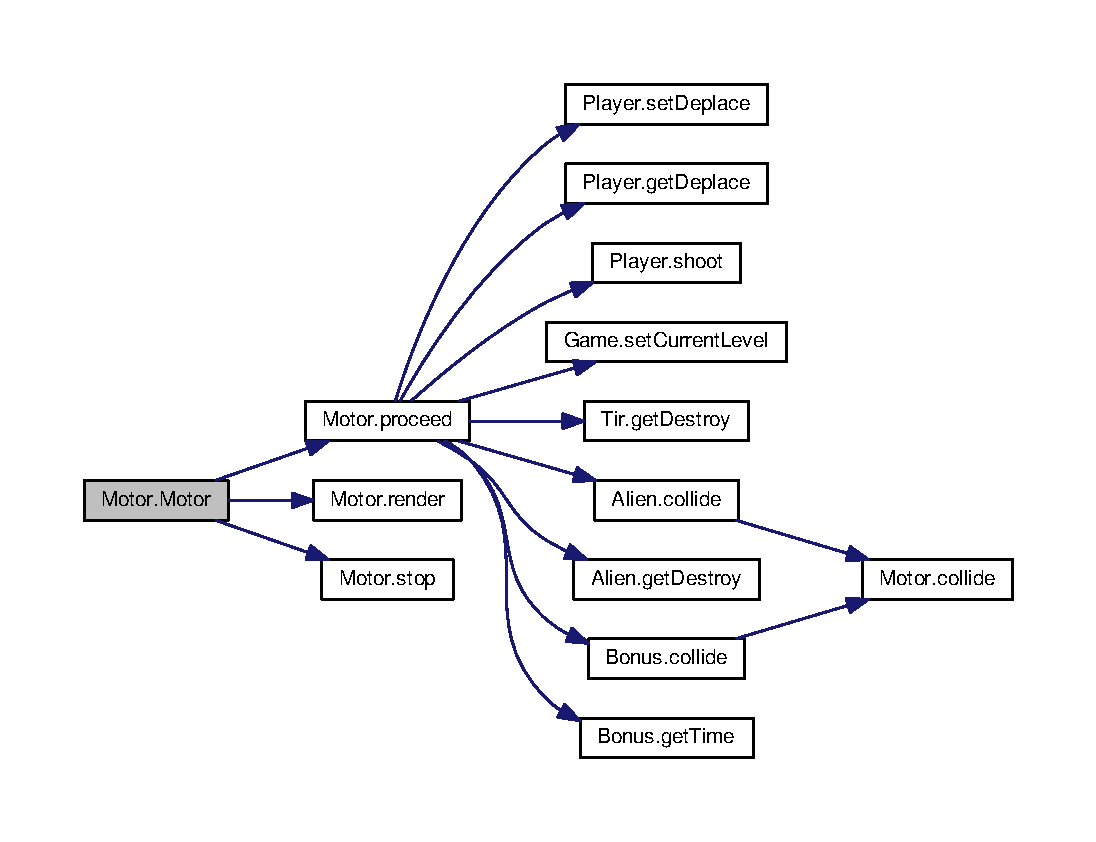
\includegraphics[width=350pt]{class_motor_ac2cb95916f7081fef0b4582db086404e_cgraph}
\end{center}
\end{figure}




\subsection{Documentation des fonctions membres}
\hypertarget{class_motor_a810690068c5edddd73d584e0dd19acd4}{\index{Motor@{Motor}!collide@{collide}}
\index{collide@{collide}!Motor@{Motor}}
\subsubsection[{collide}]{\setlength{\rightskip}{0pt plus 5cm}static Pair$<$Integer,Integer$>$ Motor.\-collide (
\begin{DoxyParamCaption}
\item[{int}]{x1, }
\item[{int}]{y1, }
\item[{Image}]{img1, }
\item[{int}]{x2, }
\item[{int}]{y2, }
\item[{Image}]{img2}
\end{DoxyParamCaption}
)\hspace{0.3cm}{\ttfamily [static]}}}\label{class_motor_a810690068c5edddd73d584e0dd19acd4}


Methode générale de detection de collision entre deux objets. 

Le but est de considérer une collision comme une zone commune à deux entités. La zone est parcourue une fois et les pixels des deux entités contenus dans cette zone sont comparés. Si les deux pixels des deux entités ne sont pas transparant, alors il y une collision entre les deux entités 
\begin{DoxyItemize}
\item Test de collision simple \-: on regarde si les zones des deux entités se chevauchent
\item Calcul des coordonnées absolues de la zone d'intersection
\item Chargement des pixels des deux images comparées
\item Lecture en y de la zone d'intersection
\item Lecture en x de la zone d'intersection
\item Récupération du pixel relatif à la première image
\item Récupération du pixel relatif à la deuxième image
\item Collision détectée \-: on renvoit la position absolue de la collision 
\end{DoxyItemize}

Définition à la ligne 298 du fichier Motor.\-java.



Voici le graphe des appelants de cette fonction \-:
\nopagebreak
\begin{figure}[H]
\begin{center}
\leavevmode
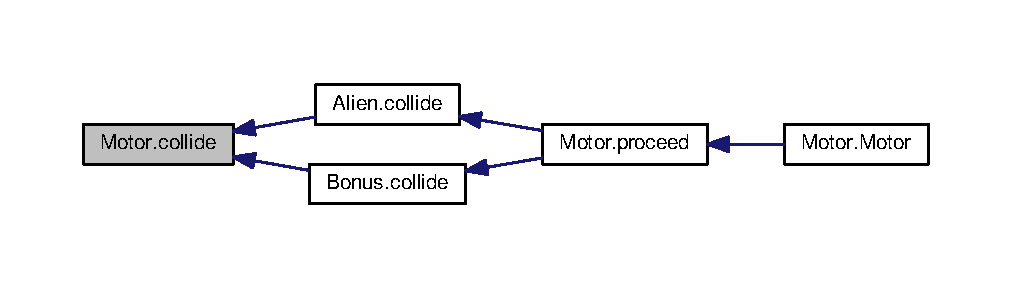
\includegraphics[width=350pt]{class_motor_a810690068c5edddd73d584e0dd19acd4_icgraph}
\end{center}
\end{figure}


\hypertarget{class_motor_a33b87f33f275b9f87ed7791857af2cf3}{\index{Motor@{Motor}!get\-Active\-Bonus@{get\-Active\-Bonus}}
\index{get\-Active\-Bonus@{get\-Active\-Bonus}!Motor@{Motor}}
\subsubsection[{get\-Active\-Bonus}]{\setlength{\rightskip}{0pt plus 5cm}Array\-List$<${\bf Bonus}$>$ Motor.\-get\-Active\-Bonus (
\begin{DoxyParamCaption}
{}
\end{DoxyParamCaption}
)}}\label{class_motor_a33b87f33f275b9f87ed7791857af2cf3}


Méthode renvoyant la liste des bonus actifs actuellement. 



Définition à la ligne 401 du fichier Motor.\-java.

\hypertarget{class_motor_a787633e0544ca8c8dceb3f415b7aeeea}{\index{Motor@{Motor}!get\-Aliens@{get\-Aliens}}
\index{get\-Aliens@{get\-Aliens}!Motor@{Motor}}
\subsubsection[{get\-Aliens}]{\setlength{\rightskip}{0pt plus 5cm}Array\-List$<${\bf Alien}$>$ Motor.\-get\-Aliens (
\begin{DoxyParamCaption}
{}
\end{DoxyParamCaption}
)}}\label{class_motor_a787633e0544ca8c8dceb3f415b7aeeea}


Méthode renvoyant la liste des aliens affichés. 



Définition à la ligne 389 du fichier Motor.\-java.

\hypertarget{class_motor_a42d5acc1b6be21bade008a427bef9c64}{\index{Motor@{Motor}!get\-Bonus@{get\-Bonus}}
\index{get\-Bonus@{get\-Bonus}!Motor@{Motor}}
\subsubsection[{get\-Bonus}]{\setlength{\rightskip}{0pt plus 5cm}Array\-List$<${\bf Bonus}$>$ Motor.\-get\-Bonus (
\begin{DoxyParamCaption}
{}
\end{DoxyParamCaption}
)}}\label{class_motor_a42d5acc1b6be21bade008a427bef9c64}


Méthode renvoyant la liste des bonus affichés. 



Définition à la ligne 395 du fichier Motor.\-java.

\hypertarget{class_motor_af1d6924fafe1e9d2ce3c77799c35a136}{\index{Motor@{Motor}!get\-Houses@{get\-Houses}}
\index{get\-Houses@{get\-Houses}!Motor@{Motor}}
\subsubsection[{get\-Houses}]{\setlength{\rightskip}{0pt plus 5cm}Array\-List$<${\bf House}$>$ Motor.\-get\-Houses (
\begin{DoxyParamCaption}
{}
\end{DoxyParamCaption}
)}}\label{class_motor_af1d6924fafe1e9d2ce3c77799c35a136}


Méthode renvoyant la liste des maisons. 



Définition à la ligne 383 du fichier Motor.\-java.

\hypertarget{class_motor_a054f1e6ac323e78270bcb2ed9687fb80}{\index{Motor@{Motor}!get\-Player@{get\-Player}}
\index{get\-Player@{get\-Player}!Motor@{Motor}}
\subsubsection[{get\-Player}]{\setlength{\rightskip}{0pt plus 5cm}{\bf Player} Motor.\-get\-Player (
\begin{DoxyParamCaption}
{}
\end{DoxyParamCaption}
)}}\label{class_motor_a054f1e6ac323e78270bcb2ed9687fb80}


Methode renvoyant l'objet joueur. 



Définition à la ligne 407 du fichier Motor.\-java.

\hypertarget{class_motor_ab31da9ce3d509a33029d6025f3596604}{\index{Motor@{Motor}!get\-Tirs@{get\-Tirs}}
\index{get\-Tirs@{get\-Tirs}!Motor@{Motor}}
\subsubsection[{get\-Tirs}]{\setlength{\rightskip}{0pt plus 5cm}Array\-List$<${\bf Tir}$>$ Motor.\-get\-Tirs (
\begin{DoxyParamCaption}
{}
\end{DoxyParamCaption}
)}}\label{class_motor_ab31da9ce3d509a33029d6025f3596604}


Méthode renvoyant la liste des missiles affichés. 



Définition à la ligne 377 du fichier Motor.\-java.

\hypertarget{class_motor_a5333ff4fde112f55953849964f8ae7fa}{\index{Motor@{Motor}!proceed@{proceed}}
\index{proceed@{proceed}!Motor@{Motor}}
\subsubsection[{proceed}]{\setlength{\rightskip}{0pt plus 5cm}void Motor.\-proceed (
\begin{DoxyParamCaption}
\item[{float}]{timestep, }
\item[{Array\-List$<$ Key\-Code $>$}]{keys}
\end{DoxyParamCaption}
)}}\label{class_motor_a5333ff4fde112f55953849964f8ae7fa}


Methode s'occupant des déplacements et changement d'état à partir des données du jeu. 

Méthode la plus importante du jeu \-: c'est elle qui s'occupe du déroulement général du jeu. Elle est appellée par la gameloop. Elle parcourt tous les éléments du jeu et s'occupe de les faire intéragir. Une méthode \hyperlink{class_motor_a5333ff4fde112f55953849964f8ae7fa}{proceed()} d'une classe peut se traduire par \char`\"{}c'est à moi de jouer, comment dois-\/je jouer ?\char`\"{}. La méthode proceed du moteur de jeu ne s'occupe pas de bouger directement les entitées, elle appelle la méthode proceed de chacune des ses entitées. Itérateus permettants de supprimer un élément d'une liste que l'on est en train de parcourir


\begin{DoxyItemize}
\item Ordonnée du dernier alien ajouté au jeu, qui sera forcément dans la ligne la plus haute
\end{DoxyItemize}

Incrémente le temps écoulé au chronomètre \char`\"{}level\-\_\-up\-\_\-time\char`\"{}. Si le chronomètre a dépassé les trente secondes, il se remet à zéro et le niveau affiché augmente de un.


\begin{DoxyItemize}
\item Met à zéro le vecteur déplacement du joueur
\item Si la flèche de gauche du clavier a été pressé depuis le dernier \hyperlink{class_motor_a5333ff4fde112f55953849964f8ae7fa}{proceed()}, décrémente de deux le vecteur de déplacement du joueur
\item Si la flèche de droite du clavier a été pressé depuis le dernier \hyperlink{class_motor_a5333ff4fde112f55953849964f8ae7fa}{proceed()}, incrémente de deux le vecteur de déplacement du joueur
\item Si la touche espace du clavier a été pressé depuis le dernier \hyperlink{class_motor_a5333ff4fde112f55953849964f8ae7fa}{proceed()}, appelle la méthode shoot() du joueur
\item Si la touche \char`\"{}\-P\char`\"{} du clavier a été pressé depuis le dernier \hyperlink{class_motor_a5333ff4fde112f55953849964f8ae7fa}{proceed()}, change l'écran de jeu par celui de pause
\end{DoxyItemize}

Appelle le procced() du joueur avec le temps écoulé depuis le dernier

Pour chaque missile, appelle son \hyperlink{class_motor_a5333ff4fde112f55953849964f8ae7fa}{proceed()} et, si son indicateur de destruction s'est mis à 1, l'enlève de la liste

Appelle le \hyperlink{class_motor_a5333ff4fde112f55953849964f8ae7fa}{proceed()} de toute la classe \hyperlink{class_alien}{Alien} avec le temps écoulé depuis le dernier

Pour chaque alien, appelle son propre \hyperlink{class_motor_a5333ff4fde112f55953849964f8ae7fa}{proceed()} Appelle la fonction \hyperlink{class_motor_a810690068c5edddd73d584e0dd19acd4}{collide()} de l'alien avec le joueur, si elle renvoie vrai, retire toutes les vies du joueur et déclanche l'écran gameover. Si l'indicateur de destruction de l'alien est à 1, le retire de la liste.


\begin{DoxyItemize}
\item Met à jour l'ordonnée de l'alien le plus haut avec les nouvelles positions des aliens qui viennent de se déplacer (à nouveau, le dernier alien ajouté dans la liste sera forcément dans la ligne la plus haute).
\end{DoxyItemize}

À chaque fois que cet ordonné dépasse 0.\-0, ajoute une nouvelle ligne d'alien 50 pixels plus haut. Les 50 représente l'écart qu'il y a entre chaque ligne d'alien. Le fait qu'une nouvelle ligne d'alien soit ajoutée dès que l'ancienne dépasse 0.\-0 (la nouvelle ligne d'alien est dessinée hors-\/cadre) permet de faire en sorte que les aliens sorte graduellement du haut de l'écran plutôt que d'apparaître d'un coup. La valeur d'index\-\_\-alien est incrémentée à chaque nouvelle ligne pour faire en sorte que la prochain soit du type d'alien qui suit (la valeur revient à 0 au lieu de passer à 5 pour ne pas sortir de la liste d'images). On vérifie également avant tout que la liste d'aliens n'est pas vide pour parer à toutes éventualité. Si cette liste est vide, \char`\"{}y\-\_\-last\-\_\-alien\char`\"{} prend la valeur 14.\-0 car la hauteur des images d'alien est de 36px donc, puisque la nouvelle ligne sera dessiné à l'ordonnée \char`\"{}y\-\_\-last\-\_\-alien\char`\"{}-\/50 (-\/36px dans ce cas), cette nouvelle ligne apparait au joueur immédiatement après la disparition du dernier alien.

Pour chaque bonus affiché, appelle son \hyperlink{class_motor_a5333ff4fde112f55953849964f8ae7fa}{proceed()}, vérifie si une collision a eu lieu avec le joueur (si c'est le cas appelle la méthode active() du bonus et l'enlève de la liste) ou si le bonus n'a pas dépassé le cadre du jeu (l'enlève simplement de la liste dans ce cas).

Pour chaque bonus en activation, ajoute le temps écoulé depuis le dernier appel à cette fonction, et si ce temps dépasse le temps d'activation maximum des bonus, appelle la méthode inactive() de ce bonus et le retire de la liste

Définition à la ligne 161 du fichier Motor.\-java.



Voici le graphe d'appel pour cette fonction \-:
\nopagebreak
\begin{figure}[H]
\begin{center}
\leavevmode
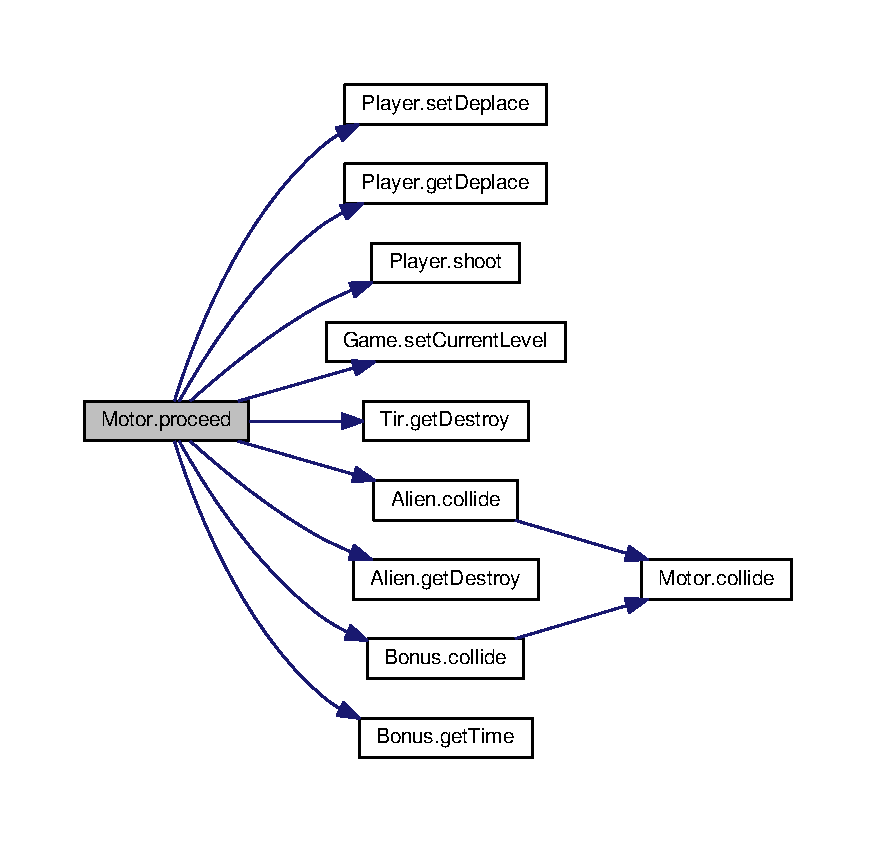
\includegraphics[width=350pt]{class_motor_a5333ff4fde112f55953849964f8ae7fa_cgraph}
\end{center}
\end{figure}




Voici le graphe des appelants de cette fonction \-:
\nopagebreak
\begin{figure}[H]
\begin{center}
\leavevmode
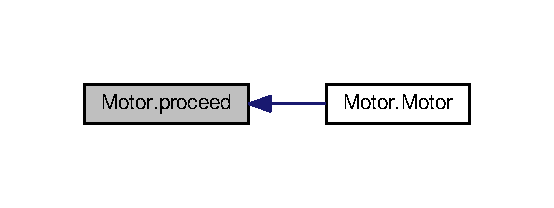
\includegraphics[width=266pt]{class_motor_a5333ff4fde112f55953849964f8ae7fa_icgraph}
\end{center}
\end{figure}


\hypertarget{class_motor_a73f2becef3f9ceb3a54b9698e8ef7d05}{\index{Motor@{Motor}!render@{render}}
\index{render@{render}!Motor@{Motor}}
\subsubsection[{render}]{\setlength{\rightskip}{0pt plus 5cm}void Motor.\-render (
\begin{DoxyParamCaption}
\item[{Graphics\-Context}]{gc}
\end{DoxyParamCaption}
)}}\label{class_motor_a73f2becef3f9ceb3a54b9698e8ef7d05}


Methode d'affichage de tout les objets du jeu. 

Un seul appel par frame 
\begin{DoxyItemize}
\item Dessine le fond dans le canvas en recouvrant tout ce qui a été dessiné avant
\item Dessine le vaisseau du joueur à sa position actuelle
\item Dessine chaque bonus à sa positions actuelle
\item Ajoute une brillance qui sera appliqué aux prochains éléments dessinés pour des raison de visibilité
\item Appelle la fonction draw() de chaque missile, qui les dessineront à leurs positions actuelles
\item Appelle la fonction draw() de chaque maison, qui la dessineront dans son état de destruction actuels
\item Change la brillance utilisé par une plus lumineuse (celui par défaut a une puissance de 0.\-3, on le passe à 0.\-5 pour les aliens uniquement)
\item Dessine chaque alien à sa positions actuelle
\item Retire l'effet de brillance du Graphic\-Context pour qu'il ne soit pas appliqué au prochain draw() sur le image qui ne doivent pas en recevoir 
\end{DoxyItemize}

Définition à la ligne 344 du fichier Motor.\-java.



Voici le graphe des appelants de cette fonction \-:
\nopagebreak
\begin{figure}[H]
\begin{center}
\leavevmode
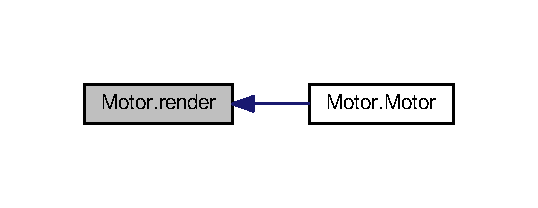
\includegraphics[width=258pt]{class_motor_a73f2becef3f9ceb3a54b9698e8ef7d05_icgraph}
\end{center}
\end{figure}


\hypertarget{class_motor_a6ae139ee985ef74ec9704b895f3b8895}{\index{Motor@{Motor}!start@{start}}
\index{start@{start}!Motor@{Motor}}
\subsubsection[{start}]{\setlength{\rightskip}{0pt plus 5cm}void Motor.\-start (
\begin{DoxyParamCaption}
{}
\end{DoxyParamCaption}
)}}\label{class_motor_a6ae139ee985ef74ec9704b895f3b8895}


Methode de lancement de la Game\-Loop. 



Définition à la ligne 51 du fichier Motor.\-java.

\hypertarget{class_motor_a9a5d81ced7a0f9d679732839a8f77d3a}{\index{Motor@{Motor}!stop@{stop}}
\index{stop@{stop}!Motor@{Motor}}
\subsubsection[{stop}]{\setlength{\rightskip}{0pt plus 5cm}void Motor.\-stop (
\begin{DoxyParamCaption}
{}
\end{DoxyParamCaption}
)}}\label{class_motor_a9a5d81ced7a0f9d679732839a8f77d3a}


Methode d'arrêt de la Game\-Loop. 



Définition à la ligne 58 du fichier Motor.\-java.



Voici le graphe des appelants de cette fonction \-:
\nopagebreak
\begin{figure}[H]
\begin{center}
\leavevmode
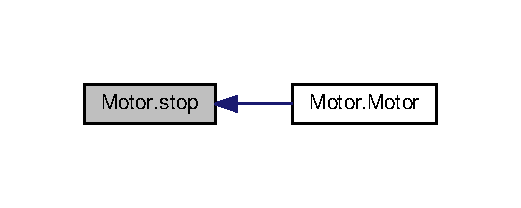
\includegraphics[width=250pt]{class_motor_a9a5d81ced7a0f9d679732839a8f77d3a_icgraph}
\end{center}
\end{figure}




La documentation de cette classe a été générée à partir du fichier suivant \-:\begin{DoxyCompactItemize}
\item 
\hyperlink{_motor_8java}{Motor.\-java}\end{DoxyCompactItemize}

\hypertarget{class_movit}{\section{Référence de la classe Movit}
\label{class_movit}\index{Movit@{Movit}}
}


Graphe d'héritage de Movit\-:
\nopagebreak
\begin{figure}[H]
\begin{center}
\leavevmode
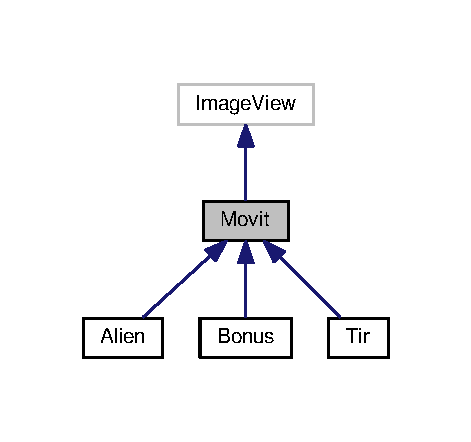
\includegraphics[width=226pt]{class_movit__inherit__graph}
\end{center}
\end{figure}


Graphe de collaboration de Movit\-:
\nopagebreak
\begin{figure}[H]
\begin{center}
\leavevmode
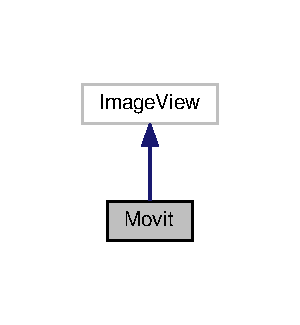
\includegraphics[width=144pt]{class_movit__coll__graph}
\end{center}
\end{figure}
\subsection*{Fonctions membres publiques}
\begin{DoxyCompactItemize}
\item 
\hyperlink{class_movit_a49b9f207b93ff26c86f63a70882e68de}{Movit} (Image img, double vecx, double vecy, double x, double y)
\begin{DoxyCompactList}\small\item\em Constructeur d'un mobile. \end{DoxyCompactList}\end{DoxyCompactItemize}
\subsection*{Fonctions membres publiques statiques}
\begin{DoxyCompactItemize}
\item 
static Image\mbox{[}$\,$\mbox{]} \hyperlink{class_movit_a274641e5ce00194f1784063cde95ab49}{imglist} (String s, byte n)
\begin{DoxyCompactList}\small\item\em Méthode créant un tableau d'images. \end{DoxyCompactList}\end{DoxyCompactItemize}
\subsection*{Attributs protégés}
\begin{DoxyCompactItemize}
\item 
double \hyperlink{class_movit_a0cd05b4b560be5799e492562f3b539c9}{vec\-X}
\begin{DoxyCompactList}\small\item\em vecteur de déplacement horizontal \end{DoxyCompactList}\item 
double \hyperlink{class_movit_abfe200611d0a57b9642337e0494ee1f9}{vec\-Y}
\begin{DoxyCompactList}\small\item\em vecteur de déplacement vertical \end{DoxyCompactList}\end{DoxyCompactItemize}


\subsection{Description détaillée}


Définition à la ligne 10 du fichier Movit.\-java.



\subsection{Documentation des constructeurs et destructeur}
\hypertarget{class_movit_a49b9f207b93ff26c86f63a70882e68de}{\index{Movit@{Movit}!Movit@{Movit}}
\index{Movit@{Movit}!Movit@{Movit}}
\subsubsection[{Movit}]{\setlength{\rightskip}{0pt plus 5cm}Movit.\-Movit (
\begin{DoxyParamCaption}
\item[{Image}]{img, }
\item[{double}]{vecx, }
\item[{double}]{vecy, }
\item[{double}]{x, }
\item[{double}]{y}
\end{DoxyParamCaption}
)}}\label{class_movit_a49b9f207b93ff26c86f63a70882e68de}


Constructeur d'un mobile. 

Appelle le constructeur d'Image\-View avec l'image donnée en paramètre (Image\-View est un objet Java\-F\-X contenant une image affichable (et réglable). Initialise les vecteurs de déplacement et positionne l'image avec les valeurs passés en argument. 

Définition à la ligne 21 du fichier Movit.\-java.



\subsection{Documentation des fonctions membres}
\hypertarget{class_movit_a274641e5ce00194f1784063cde95ab49}{\index{Movit@{Movit}!imglist@{imglist}}
\index{imglist@{imglist}!Movit@{Movit}}
\subsubsection[{imglist}]{\setlength{\rightskip}{0pt plus 5cm}static Image \mbox{[}$\,$\mbox{]} Movit.\-imglist (
\begin{DoxyParamCaption}
\item[{String}]{s, }
\item[{byte}]{n}
\end{DoxyParamCaption}
)\hspace{0.3cm}{\ttfamily [static]}}}\label{class_movit_a274641e5ce00194f1784063cde95ab49}


Méthode créant un tableau d'images. 

Cette méthode a été créée pour éviter les répétitions dans notre code car que ce soit pour les aliens ou les bonus, on doit créer une liste d'images de tous les types d'aliens/bonus possibles. Ces images sont dans les deux cas stockées dans un dossier homonyme (on leur accole un identifiant numérique pour les distinguer). Pour récupérer la liste il nous suffit d'appeler cette fonction en lui précisant un nombre d'images et le nom du dossier les contenant, cette fonction remplira la liste avec les bons chemins. 

Définition à la ligne 34 du fichier Movit.\-java.



\subsection{Documentation des données membres}
\hypertarget{class_movit_a0cd05b4b560be5799e492562f3b539c9}{\index{Movit@{Movit}!vec\-X@{vec\-X}}
\index{vec\-X@{vec\-X}!Movit@{Movit}}
\subsubsection[{vec\-X}]{\setlength{\rightskip}{0pt plus 5cm}double Movit.\-vec\-X\hspace{0.3cm}{\ttfamily [protected]}}}\label{class_movit_a0cd05b4b560be5799e492562f3b539c9}


vecteur de déplacement horizontal 


\begin{DoxyItemize}
\item 
\end{DoxyItemize}

Définition à la ligne 12 du fichier Movit.\-java.

\hypertarget{class_movit_abfe200611d0a57b9642337e0494ee1f9}{\index{Movit@{Movit}!vec\-Y@{vec\-Y}}
\index{vec\-Y@{vec\-Y}!Movit@{Movit}}
\subsubsection[{vec\-Y}]{\setlength{\rightskip}{0pt plus 5cm}double Movit.\-vec\-Y\hspace{0.3cm}{\ttfamily [protected]}}}\label{class_movit_abfe200611d0a57b9642337e0494ee1f9}


vecteur de déplacement vertical 


\begin{DoxyItemize}
\item 
\end{DoxyItemize}

Définition à la ligne 14 du fichier Movit.\-java.



La documentation de cette classe a été générée à partir du fichier suivant \-:\begin{DoxyCompactItemize}
\item 
\hyperlink{_movit_8java}{Movit.\-java}\end{DoxyCompactItemize}

\hypertarget{class_player}{\section{Référence de la classe Player}
\label{class_player}\index{Player@{Player}}
}


Graphe d'héritage de Player\-:
\nopagebreak
\begin{figure}[H]
\begin{center}
\leavevmode
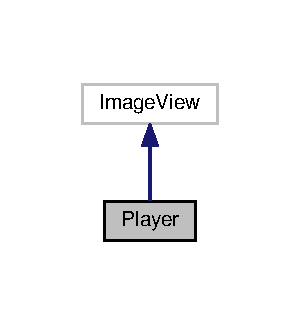
\includegraphics[width=144pt]{class_player__inherit__graph}
\end{center}
\end{figure}


Graphe de collaboration de Player\-:
\nopagebreak
\begin{figure}[H]
\begin{center}
\leavevmode
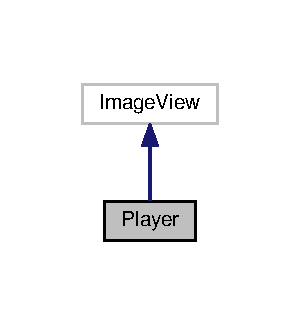
\includegraphics[width=144pt]{class_player__coll__graph}
\end{center}
\end{figure}
\subsection*{Fonctions membres publiques}
\begin{DoxyCompactItemize}
\item 
\hyperlink{class_player_a712a726b07cf901c040116d6d0c5cc66}{Player} ()
\begin{DoxyCompactList}\small\item\em Constructeur du joueur. \end{DoxyCompactList}\item 
void \hyperlink{class_player_a9a32aeb96a7184620e3342244e6d17ad}{proceed} (float timestep)
\begin{DoxyCompactList}\small\item\em Methode actualisant la position de \hyperlink{class_player}{Player}. \end{DoxyCompactList}\item 
void \hyperlink{class_player_adff9fbff40a2ad4a8fa2b89884e6e7d2}{shoot} ()
\begin{DoxyCompactList}\small\item\em Methode de tir du joueur. \end{DoxyCompactList}\item 
void \hyperlink{class_player_acab62e8dde064015d176aae75fdcd263}{destruct} ()
\begin{DoxyCompactList}\small\item\em Methode appelée en cas de collision entre le joueur et un missile. \end{DoxyCompactList}\item 
double \hyperlink{class_player_acce5669fa54c5a76c5e69ad890ded0a6}{get\-Deplace} ()
\begin{DoxyCompactList}\small\item\em Methode renvoyant le vecteur de déplacement. \end{DoxyCompactList}\item 
void \hyperlink{class_player_ae3de1d7541e006a1835428ea05d8ac5c}{set\-Deplace} (double pas)
\begin{DoxyCompactList}\small\item\em Methode paramètrant le vecteur de deplacement. \end{DoxyCompactList}\item 
float \hyperlink{class_player_af3f440fabf4174f321e854ff8fabd25a}{get\-Delay\-Tir} ()
\begin{DoxyCompactList}\small\item\em Methode renvoyant le delai minimum entre deux tirs. \end{DoxyCompactList}\item 
void \hyperlink{class_player_a1f3118b8d157fe53c585318d4914fc08}{set\-Delay\-Tir} (float delay)
\begin{DoxyCompactList}\small\item\em Methode paramétrant le delai minimum entre deux tirs. \end{DoxyCompactList}\item 
double \hyperlink{class_player_a1e53e9e10195f64b4ae551747245c7f2}{get\-Vitesse\-Tir} ()
\begin{DoxyCompactList}\small\item\em Methode renvoyant la vitesse d'un missile tiré \end{DoxyCompactList}\item 
void \hyperlink{class_player_a884976391b424945d77108463de3b2b8}{set\-Vitesse\-Tir} (double vitesse)
\begin{DoxyCompactList}\small\item\em Methode paramétrant la vitesse d'un missile tiré \end{DoxyCompactList}\end{DoxyCompactItemize}


\subsection{Description détaillée}


Définition à la ligne 13 du fichier Player.\-java.



\subsection{Documentation des constructeurs et destructeur}
\hypertarget{class_player_a712a726b07cf901c040116d6d0c5cc66}{\index{Player@{Player}!Player@{Player}}
\index{Player@{Player}!Player@{Player}}
\subsubsection[{Player}]{\setlength{\rightskip}{0pt plus 5cm}Player.\-Player (
\begin{DoxyParamCaption}
{}
\end{DoxyParamCaption}
)}}\label{class_player_a712a726b07cf901c040116d6d0c5cc66}


Constructeur du joueur. 

Appelle le constructeur d'Image\-View avec l'image du vaisseau du joueur. Initialise les deux sons associés au joueur. Place le joueur en bas et au milieu horizontalement de l'écran. Initialise les vecteurs, délai et chronomètre à leur valeur de départ. \hyperlink{class_player}{Player} n'hérite pas de \hyperlink{class_movit}{Movit} car il ne possède pas de vecteur de déplacement vertical et qu'on a besoin d'utiliser relocate() après avoir défini son image. 

Définition à la ligne 37 du fichier Player.\-java.



\subsection{Documentation des fonctions membres}
\hypertarget{class_player_acab62e8dde064015d176aae75fdcd263}{\index{Player@{Player}!destruct@{destruct}}
\index{destruct@{destruct}!Player@{Player}}
\subsubsection[{destruct}]{\setlength{\rightskip}{0pt plus 5cm}void Player.\-destruct (
\begin{DoxyParamCaption}
{}
\end{DoxyParamCaption}
)}}\label{class_player_acab62e8dde064015d176aae75fdcd263}


Methode appelée en cas de collision entre le joueur et un missile. 

Joue le son de collision entre le joueur et un missile. Retire une vie au joueur et, s'il n'en a plus, met le jeu sur l'écran de gameover. 

Définition à la ligne 91 du fichier Player.\-java.

\hypertarget{class_player_af3f440fabf4174f321e854ff8fabd25a}{\index{Player@{Player}!get\-Delay\-Tir@{get\-Delay\-Tir}}
\index{get\-Delay\-Tir@{get\-Delay\-Tir}!Player@{Player}}
\subsubsection[{get\-Delay\-Tir}]{\setlength{\rightskip}{0pt plus 5cm}float Player.\-get\-Delay\-Tir (
\begin{DoxyParamCaption}
{}
\end{DoxyParamCaption}
)}}\label{class_player_af3f440fabf4174f321e854ff8fabd25a}


Methode renvoyant le delai minimum entre deux tirs. 



Définition à la ligne 113 du fichier Player.\-java.

\hypertarget{class_player_acce5669fa54c5a76c5e69ad890ded0a6}{\index{Player@{Player}!get\-Deplace@{get\-Deplace}}
\index{get\-Deplace@{get\-Deplace}!Player@{Player}}
\subsubsection[{get\-Deplace}]{\setlength{\rightskip}{0pt plus 5cm}double Player.\-get\-Deplace (
\begin{DoxyParamCaption}
{}
\end{DoxyParamCaption}
)}}\label{class_player_acce5669fa54c5a76c5e69ad890ded0a6}


Methode renvoyant le vecteur de déplacement. 



Définition à la ligne 101 du fichier Player.\-java.



Voici le graphe des appelants de cette fonction \-:
\nopagebreak
\begin{figure}[H]
\begin{center}
\leavevmode
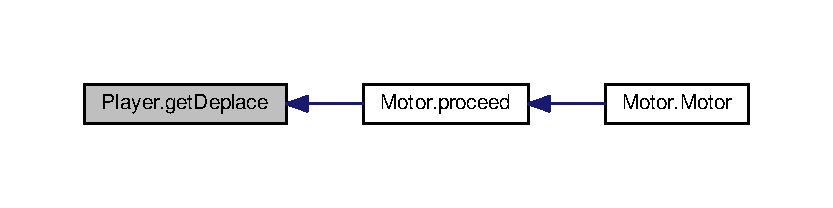
\includegraphics[width=350pt]{class_player_acce5669fa54c5a76c5e69ad890ded0a6_icgraph}
\end{center}
\end{figure}


\hypertarget{class_player_a1e53e9e10195f64b4ae551747245c7f2}{\index{Player@{Player}!get\-Vitesse\-Tir@{get\-Vitesse\-Tir}}
\index{get\-Vitesse\-Tir@{get\-Vitesse\-Tir}!Player@{Player}}
\subsubsection[{get\-Vitesse\-Tir}]{\setlength{\rightskip}{0pt plus 5cm}double Player.\-get\-Vitesse\-Tir (
\begin{DoxyParamCaption}
{}
\end{DoxyParamCaption}
)}}\label{class_player_a1e53e9e10195f64b4ae551747245c7f2}


Methode renvoyant la vitesse d'un missile tiré 



Définition à la ligne 125 du fichier Player.\-java.

\hypertarget{class_player_a9a32aeb96a7184620e3342244e6d17ad}{\index{Player@{Player}!proceed@{proceed}}
\index{proceed@{proceed}!Player@{Player}}
\subsubsection[{proceed}]{\setlength{\rightskip}{0pt plus 5cm}void Player.\-proceed (
\begin{DoxyParamCaption}
\item[{float}]{timestep}
\end{DoxyParamCaption}
)}}\label{class_player_a9a32aeb96a7184620e3342244e6d17ad}


Methode actualisant la position de \hyperlink{class_player}{Player}. 

Enlève le temps écoulé depuis le dernier \hyperlink{class_player_a9a32aeb96a7184620e3342244e6d17ad}{proceed()} à \char`\"{}current\-\_\-delay\char`\"{} (borné à 0). Actualise la position du joueur en l'empéchant de disparaître du cadre du jeu. Si le joueur sors du cadre en ajoutant le vecteur de déplacement à la position actuelle, alors on le positionne à la limite. 

Définition à la ligne 55 du fichier Player.\-java.

\hypertarget{class_player_a1f3118b8d157fe53c585318d4914fc08}{\index{Player@{Player}!set\-Delay\-Tir@{set\-Delay\-Tir}}
\index{set\-Delay\-Tir@{set\-Delay\-Tir}!Player@{Player}}
\subsubsection[{set\-Delay\-Tir}]{\setlength{\rightskip}{0pt plus 5cm}void Player.\-set\-Delay\-Tir (
\begin{DoxyParamCaption}
\item[{float}]{delay}
\end{DoxyParamCaption}
)}}\label{class_player_a1f3118b8d157fe53c585318d4914fc08}


Methode paramétrant le delai minimum entre deux tirs. 



Définition à la ligne 119 du fichier Player.\-java.

\hypertarget{class_player_ae3de1d7541e006a1835428ea05d8ac5c}{\index{Player@{Player}!set\-Deplace@{set\-Deplace}}
\index{set\-Deplace@{set\-Deplace}!Player@{Player}}
\subsubsection[{set\-Deplace}]{\setlength{\rightskip}{0pt plus 5cm}void Player.\-set\-Deplace (
\begin{DoxyParamCaption}
\item[{double}]{pas}
\end{DoxyParamCaption}
)}}\label{class_player_ae3de1d7541e006a1835428ea05d8ac5c}


Methode paramètrant le vecteur de deplacement. 



Définition à la ligne 107 du fichier Player.\-java.



Voici le graphe des appelants de cette fonction \-:
\nopagebreak
\begin{figure}[H]
\begin{center}
\leavevmode
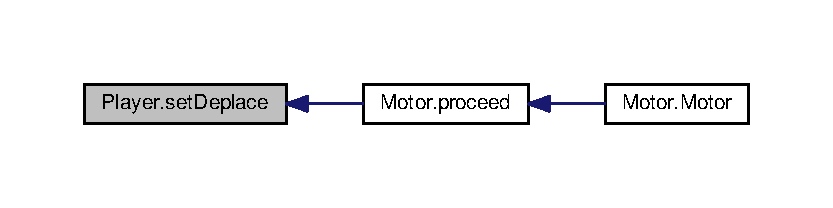
\includegraphics[width=350pt]{class_player_ae3de1d7541e006a1835428ea05d8ac5c_icgraph}
\end{center}
\end{figure}


\hypertarget{class_player_a884976391b424945d77108463de3b2b8}{\index{Player@{Player}!set\-Vitesse\-Tir@{set\-Vitesse\-Tir}}
\index{set\-Vitesse\-Tir@{set\-Vitesse\-Tir}!Player@{Player}}
\subsubsection[{set\-Vitesse\-Tir}]{\setlength{\rightskip}{0pt plus 5cm}void Player.\-set\-Vitesse\-Tir (
\begin{DoxyParamCaption}
\item[{double}]{vitesse}
\end{DoxyParamCaption}
)}}\label{class_player_a884976391b424945d77108463de3b2b8}


Methode paramétrant la vitesse d'un missile tiré 



Définition à la ligne 131 du fichier Player.\-java.

\hypertarget{class_player_adff9fbff40a2ad4a8fa2b89884e6e7d2}{\index{Player@{Player}!shoot@{shoot}}
\index{shoot@{shoot}!Player@{Player}}
\subsubsection[{shoot}]{\setlength{\rightskip}{0pt plus 5cm}void Player.\-shoot (
\begin{DoxyParamCaption}
{}
\end{DoxyParamCaption}
)}}\label{class_player_adff9fbff40a2ad4a8fa2b89884e6e7d2}


Methode de tir du joueur. 

Si le délai minimum entre deux tirs n'est pas encore écoulé, ne fais rien. Sinon, joue le son du tir, réinitialise le délai minimum, et ajoute un nouveau tir à la liste des tirs en appelant le constructeur de Tire en fonction de la position du joueur et de sa vitesse de tir. 

Définition à la ligne 77 du fichier Player.\-java.



Voici le graphe des appelants de cette fonction \-:
\nopagebreak
\begin{figure}[H]
\begin{center}
\leavevmode
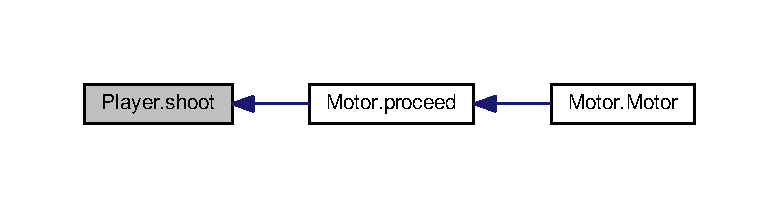
\includegraphics[width=350pt]{class_player_adff9fbff40a2ad4a8fa2b89884e6e7d2_icgraph}
\end{center}
\end{figure}




La documentation de cette classe a été générée à partir du fichier suivant \-:\begin{DoxyCompactItemize}
\item 
\hyperlink{_player_8java}{Player.\-java}\end{DoxyCompactItemize}

\hypertarget{class_tir}{\section{Référence de la classe Tir}
\label{class_tir}\index{Tir@{Tir}}
}


Graphe d'héritage de Tir\-:
\nopagebreak
\begin{figure}[H]
\begin{center}
\leavevmode
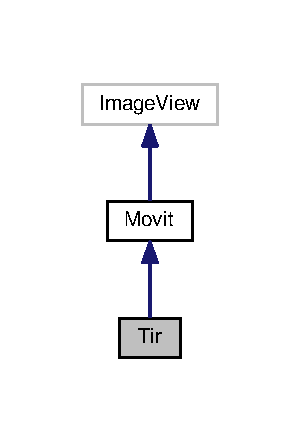
\includegraphics[width=144pt]{class_tir__inherit__graph}
\end{center}
\end{figure}


Graphe de collaboration de Tir\-:
\nopagebreak
\begin{figure}[H]
\begin{center}
\leavevmode
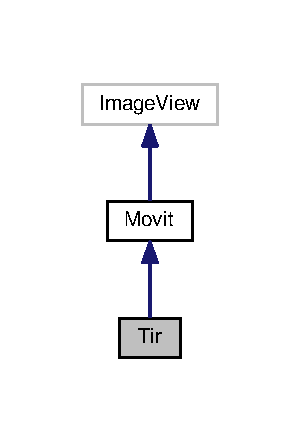
\includegraphics[width=144pt]{class_tir__coll__graph}
\end{center}
\end{figure}
\subsection*{Fonctions membres publiques}
\begin{DoxyCompactItemize}
\item 
\hyperlink{class_tir_a8841debca4a61907e5837346d864886c}{Tir} (byte index, double vecx, double vecy, double x, double y)
\begin{DoxyCompactList}\small\item\em Constructeur d'un missile. \end{DoxyCompactList}\item 
Boolean \hyperlink{class_tir_a46f4dcb5816374e482b88f371048ff37}{deplace} (double x, double y)
\begin{DoxyCompactList}\small\item\em Methode de déplacement du missile utilisée par la méthode go() \end{DoxyCompactList}\item 
void \hyperlink{class_tir_a0b2df8832aa86ef2ba9a5835fe2b99fe}{proceed} ()
\begin{DoxyCompactList}\small\item\em Methode effectuant le deplacement des objets missiles. \end{DoxyCompactList}\item 
void \hyperlink{class_tir_a7c05e3f344068c7cc9cd802d0e5beefe}{draw} (Graphics\-Context gc)
\begin{DoxyCompactList}\small\item\em Methode d'affichage d'un missile. \end{DoxyCompactList}\item 
Boolean \hyperlink{class_tir_a9e55e211b9e34cd50e32fae6f066eb7c}{get\-Destroy} ()
\begin{DoxyCompactList}\small\item\em Méthode renvoyant le drapeau indiquant si l'alien doit être détruit. \end{DoxyCompactList}\end{DoxyCompactItemize}
\subsection*{Membres hérités additionnels}


\subsection{Description détaillée}


Définition à la ligne 16 du fichier Tir.\-java.



\subsection{Documentation des constructeurs et destructeur}
\hypertarget{class_tir_a8841debca4a61907e5837346d864886c}{\index{Tir@{Tir}!Tir@{Tir}}
\index{Tir@{Tir}!Tir@{Tir}}
\subsubsection[{Tir}]{\setlength{\rightskip}{0pt plus 5cm}Tir.\-Tir (
\begin{DoxyParamCaption}
\item[{byte}]{index, }
\item[{double}]{vecx, }
\item[{double}]{vecy, }
\item[{double}]{x, }
\item[{double}]{y}
\end{DoxyParamCaption}
)}}\label{class_tir_a8841debca4a61907e5837346d864886c}


Constructeur d'un missile. 

Initialise l'image, les vecteurs et les position de départ des missiles à l'aide du constructeur de \hyperlink{class_movit}{Movit}. Si le vecteur de déplacement vertical est positif, (le missile se déplace vers le bas car il a été tiré par un alien), le missile est repositionné pour le mettre au centre par rapport à la largeur de son image, ce que la méthode shoot() de \hyperlink{class_player}{Player} ou de \hyperlink{class_alien}{Alien} ne peut pas faire sans connaissance des dimensions du missile. Elle renverse ensuite l'image du missile afin qu'il soit dessiné dans le bon sens sans avoir eu besoin de crée une image par direction. Si le missile tiré par le joueur se dirige vers le haut (tiré par le joueur), il est repositionné pour être au dessus et au centre du vaisseau du joueur (en utilisant les dimention du missile). 

Définition à la ligne 30 du fichier Tir.\-java.



\subsection{Documentation des fonctions membres}
\hypertarget{class_tir_a46f4dcb5816374e482b88f371048ff37}{\index{Tir@{Tir}!deplace@{deplace}}
\index{deplace@{deplace}!Tir@{Tir}}
\subsubsection[{deplace}]{\setlength{\rightskip}{0pt plus 5cm}Boolean Tir.\-deplace (
\begin{DoxyParamCaption}
\item[{double}]{x, }
\item[{double}]{y}
\end{DoxyParamCaption}
)}}\label{class_tir_a46f4dcb5816374e482b88f371048ff37}


Methode de déplacement du missile utilisée par la méthode go() 

Cette médhode est appellée pour chaque pixel parcouru par le missile. Le but est tester les collisions sur chaque entité du jeu (y compris les bords). On teste les collisions en utilisant la méthode de collision générale collide() de \hyperlink{class_motor}{Motor}. S'il y a une collision, la fonction détruit le missile. La gestion de collision pour chaque entité est gérée dans les fonctions collide(). Le retour de cette méthode permettra à go() de s'arrêter. 
\begin{DoxyItemize}
\item Mise à jour de la position du missile
\item Test de collision avec le joueur
\item Test de collision avec les maisons
\item Test de collision avec les aliens
\item Test de collision avec les bords du terrain 
\end{DoxyItemize}

Définition à la ligne 117 du fichier Tir.\-java.



Voici le graphe d'appel pour cette fonction \-:
\nopagebreak
\begin{figure}[H]
\begin{center}
\leavevmode
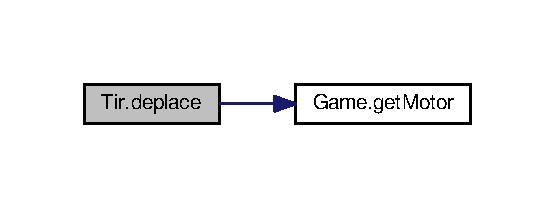
\includegraphics[width=266pt]{class_tir_a46f4dcb5816374e482b88f371048ff37_cgraph}
\end{center}
\end{figure}


\hypertarget{class_tir_a7c05e3f344068c7cc9cd802d0e5beefe}{\index{Tir@{Tir}!draw@{draw}}
\index{draw@{draw}!Tir@{Tir}}
\subsubsection[{draw}]{\setlength{\rightskip}{0pt plus 5cm}void Tir.\-draw (
\begin{DoxyParamCaption}
\item[{Graphics\-Context}]{gc}
\end{DoxyParamCaption}
)}}\label{class_tir_a7c05e3f344068c7cc9cd802d0e5beefe}


Methode d'affichage d'un missile. 



Définition à la ligne 208 du fichier Tir.\-java.

\hypertarget{class_tir_a9e55e211b9e34cd50e32fae6f066eb7c}{\index{Tir@{Tir}!get\-Destroy@{get\-Destroy}}
\index{get\-Destroy@{get\-Destroy}!Tir@{Tir}}
\subsubsection[{get\-Destroy}]{\setlength{\rightskip}{0pt plus 5cm}Boolean Tir.\-get\-Destroy (
\begin{DoxyParamCaption}
{}
\end{DoxyParamCaption}
)}}\label{class_tir_a9e55e211b9e34cd50e32fae6f066eb7c}


Méthode renvoyant le drapeau indiquant si l'alien doit être détruit. 



Définition à la ligne 214 du fichier Tir.\-java.



Voici le graphe des appelants de cette fonction \-:
\nopagebreak
\begin{figure}[H]
\begin{center}
\leavevmode
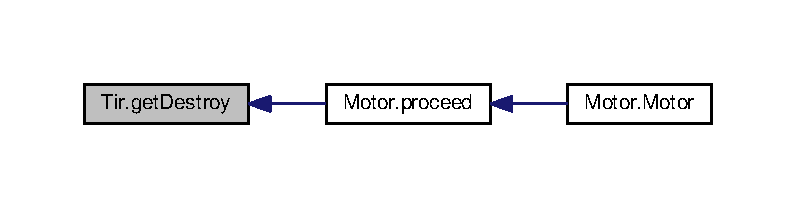
\includegraphics[width=350pt]{class_tir_a9e55e211b9e34cd50e32fae6f066eb7c_icgraph}
\end{center}
\end{figure}


\hypertarget{class_tir_a0b2df8832aa86ef2ba9a5835fe2b99fe}{\index{Tir@{Tir}!proceed@{proceed}}
\index{proceed@{proceed}!Tir@{Tir}}
\subsubsection[{proceed}]{\setlength{\rightskip}{0pt plus 5cm}void Tir.\-proceed (
\begin{DoxyParamCaption}
{}
\end{DoxyParamCaption}
)}}\label{class_tir_a0b2df8832aa86ef2ba9a5835fe2b99fe}


Methode effectuant le deplacement des objets missiles. 

Appelle la méthode go() avec les positions de départ et d'arrivée du missile. 

Définition à la ligne 201 du fichier Tir.\-java.



La documentation de cette classe a été générée à partir du fichier suivant \-:\begin{DoxyCompactItemize}
\item 
\hyperlink{_tir_8java}{Tir.\-java}\end{DoxyCompactItemize}

\chapter{Documentation des fichiers}
\hypertarget{_alien_8java}{\section{Référence du fichier Alien.\-java}
\label{_alien_8java}\index{Alien.\-java@{Alien.\-java}}
}
\subsection*{Classes}
\begin{DoxyCompactItemize}
\item 
class \hyperlink{class_alien}{Alien}
\end{DoxyCompactItemize}

\hypertarget{_bonus_8java}{\section{Référence du fichier Bonus.\-java}
\label{_bonus_8java}\index{Bonus.\-java@{Bonus.\-java}}
}
\subsection*{Classes}
\begin{DoxyCompactItemize}
\item 
class \hyperlink{class_bonus}{Bonus}
\end{DoxyCompactItemize}

\hypertarget{_game_8java}{\section{Référence du fichier Game.\-java}
\label{_game_8java}\index{Game.\-java@{Game.\-java}}
}
\subsection*{Classes}
\begin{DoxyCompactItemize}
\item 
class \hyperlink{class_game}{Game}
\end{DoxyCompactItemize}

\hypertarget{_house_8java}{\section{Référence du fichier House.\-java}
\label{_house_8java}\index{House.\-java@{House.\-java}}
}
\subsection*{Classes}
\begin{DoxyCompactItemize}
\item 
class \hyperlink{class_house}{House}
\end{DoxyCompactItemize}

\hypertarget{_motor_8java}{\section{Référence du fichier Motor.\-java}
\label{_motor_8java}\index{Motor.\-java@{Motor.\-java}}
}
\subsection*{Classes}
\begin{DoxyCompactItemize}
\item 
class \hyperlink{class_motor}{Motor}
\end{DoxyCompactItemize}

\hypertarget{_movit_8java}{\section{Référence du fichier Movit.\-java}
\label{_movit_8java}\index{Movit.\-java@{Movit.\-java}}
}
\subsection*{Classes}
\begin{DoxyCompactItemize}
\item 
class \hyperlink{class_movit}{Movit}
\end{DoxyCompactItemize}

\hypertarget{_player_8java}{\section{Référence du fichier Player.\-java}
\label{_player_8java}\index{Player.\-java@{Player.\-java}}
}
\subsection*{Classes}
\begin{DoxyCompactItemize}
\item 
class \hyperlink{class_player}{Player}
\end{DoxyCompactItemize}

\hypertarget{_tir_8java}{\section{Référence du fichier Tir.\-java}
\label{_tir_8java}\index{Tir.\-java@{Tir.\-java}}
}
\subsection*{Classes}
\begin{DoxyCompactItemize}
\item 
class \hyperlink{class_tir}{Tir}
\end{DoxyCompactItemize}

%--- End generated contents ---

% Index
\newpage
\phantomsection
\addcontentsline{toc}{chapter}{Index}
\printindex

\end{document}
